\documentclass[a4paper,12]{article}
\usepackage[latin1]{inputenc}
\usepackage[english]{babel}
\usepackage{amsmath}
\usepackage{amsfonts}
\usepackage{amssymb}
\usepackage{hyperref}
\usepackage{float}
\usepackage{adjustbox}
\usepackage{multicol}
\usepackage{caption}
\usepackage{subfiles}
\graphicspath{{Images/}{../images/}}
%Header and Footer Stuff
\usepackage{fancyhdr}
\pagestyle{fancy}
\fancyfoot{}
\fancyhead{}
\fancyfoot[R]{\thepage\ }
\renewcommand{\headrulewidth}{2pt}
\renewcommand{\footrulewidth}{2pt}
\fancyhead[L]{Class:Eng 260}
\fancyhead[R]{Hadi Asemi}
\newlength\FHoffset
\setlength\FHoffset{1cm}
\addtolength\headwidth{2\FHoffset}
\fancyheadoffset{\FHoffset}
\fancyfootoffset{\FHoffset}
% item numbering
\usepackage{enumerate}
%
\usepackage{etoolbox}
\AtBeginEnvironment{gather}{\setcounter{equation}{0}}
\AtBeginEnvironment{align}{\setcounter{equation}{0}}
\usepackage{graphicx}
\usepackage{flafter}
\usepackage{booktabs}
\usepackage{float}
\usepackage{fltrace}
\usepackage[left=2cm,right=2cm,top=2cm,bottom=2cm]{geometry}
\begin{document}
%first page title
\begin{titlepage}
	\begin{center}
		\line(1,0){300}\\
		[0.25in]
		\huge{\bfseries Eng 260}\\
		[2mm]
		\line(1,0){300}\\
		[1.5cm]
		\textsc{\LARGE Circuits}\\
		[5cm]
		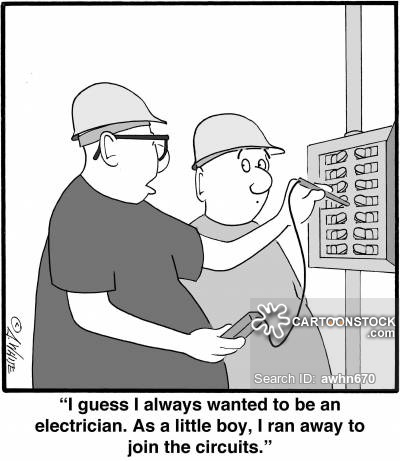
\includegraphics[width=70mm]{Image/7.jpg}
		\textsc{\Large }\\
		[4cm]
		
	\end{center}
	\begin{flushright}
		\textsc{\large Hadi Asemi\\
		Circuits\\
		 %G01049243\\
		Jan 27,2019\\}
	\end{flushright}
\end{titlepage}
	
\cleardoublepage
\tableofcontents
\thispagestyle{empty}
\cleardoublepage
\setcounter{page}{1}
\section{Circuit Analysis:}
\subsection{Basics Law}
\textbf{Example 1:}
\begin{figure}[!h]
\centering
	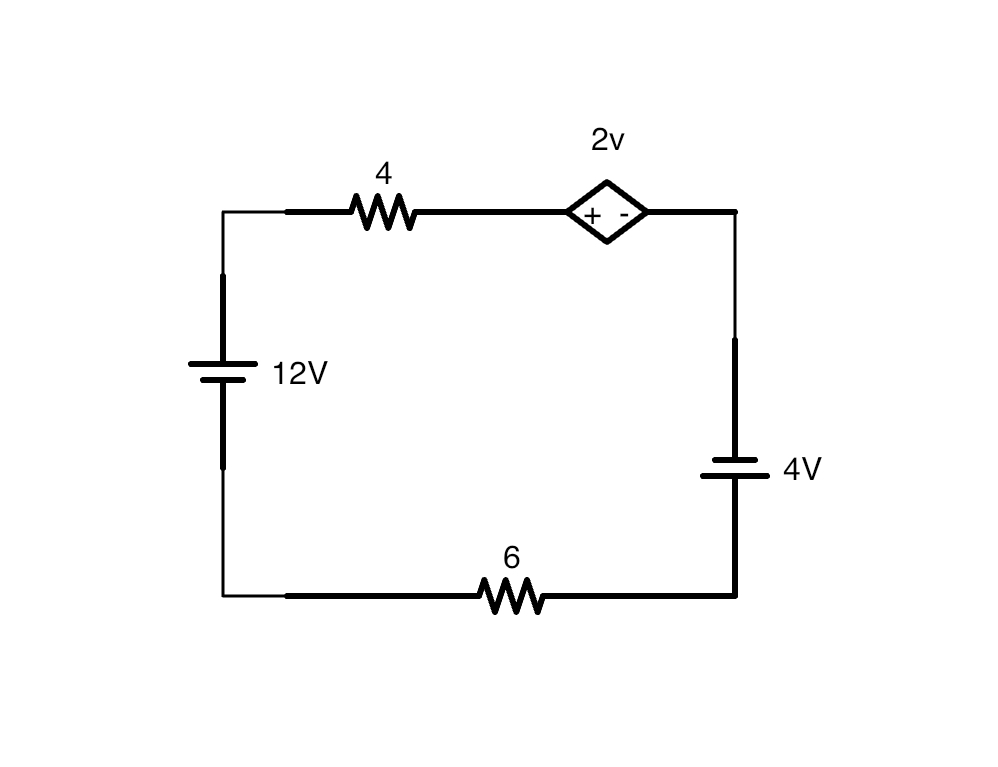
\includegraphics[width=90mm]{Image/IMG_6BA85753A355-1.jpeg}
\end{figure}
\begin{gather}
	12-4I-2v_0+4-6I=0\\
	I=\frac{v}{R}=\frac{-v_0}{6}\rightarrow v_0=-6I\\
	12-4I-2(-6I)+4-6I=0\\
	2I=-16\\
	I=8A  \indent v0=42v
\end{gather}
\textbf{Example 2:}
\begin{figure}[H]
	\centering
	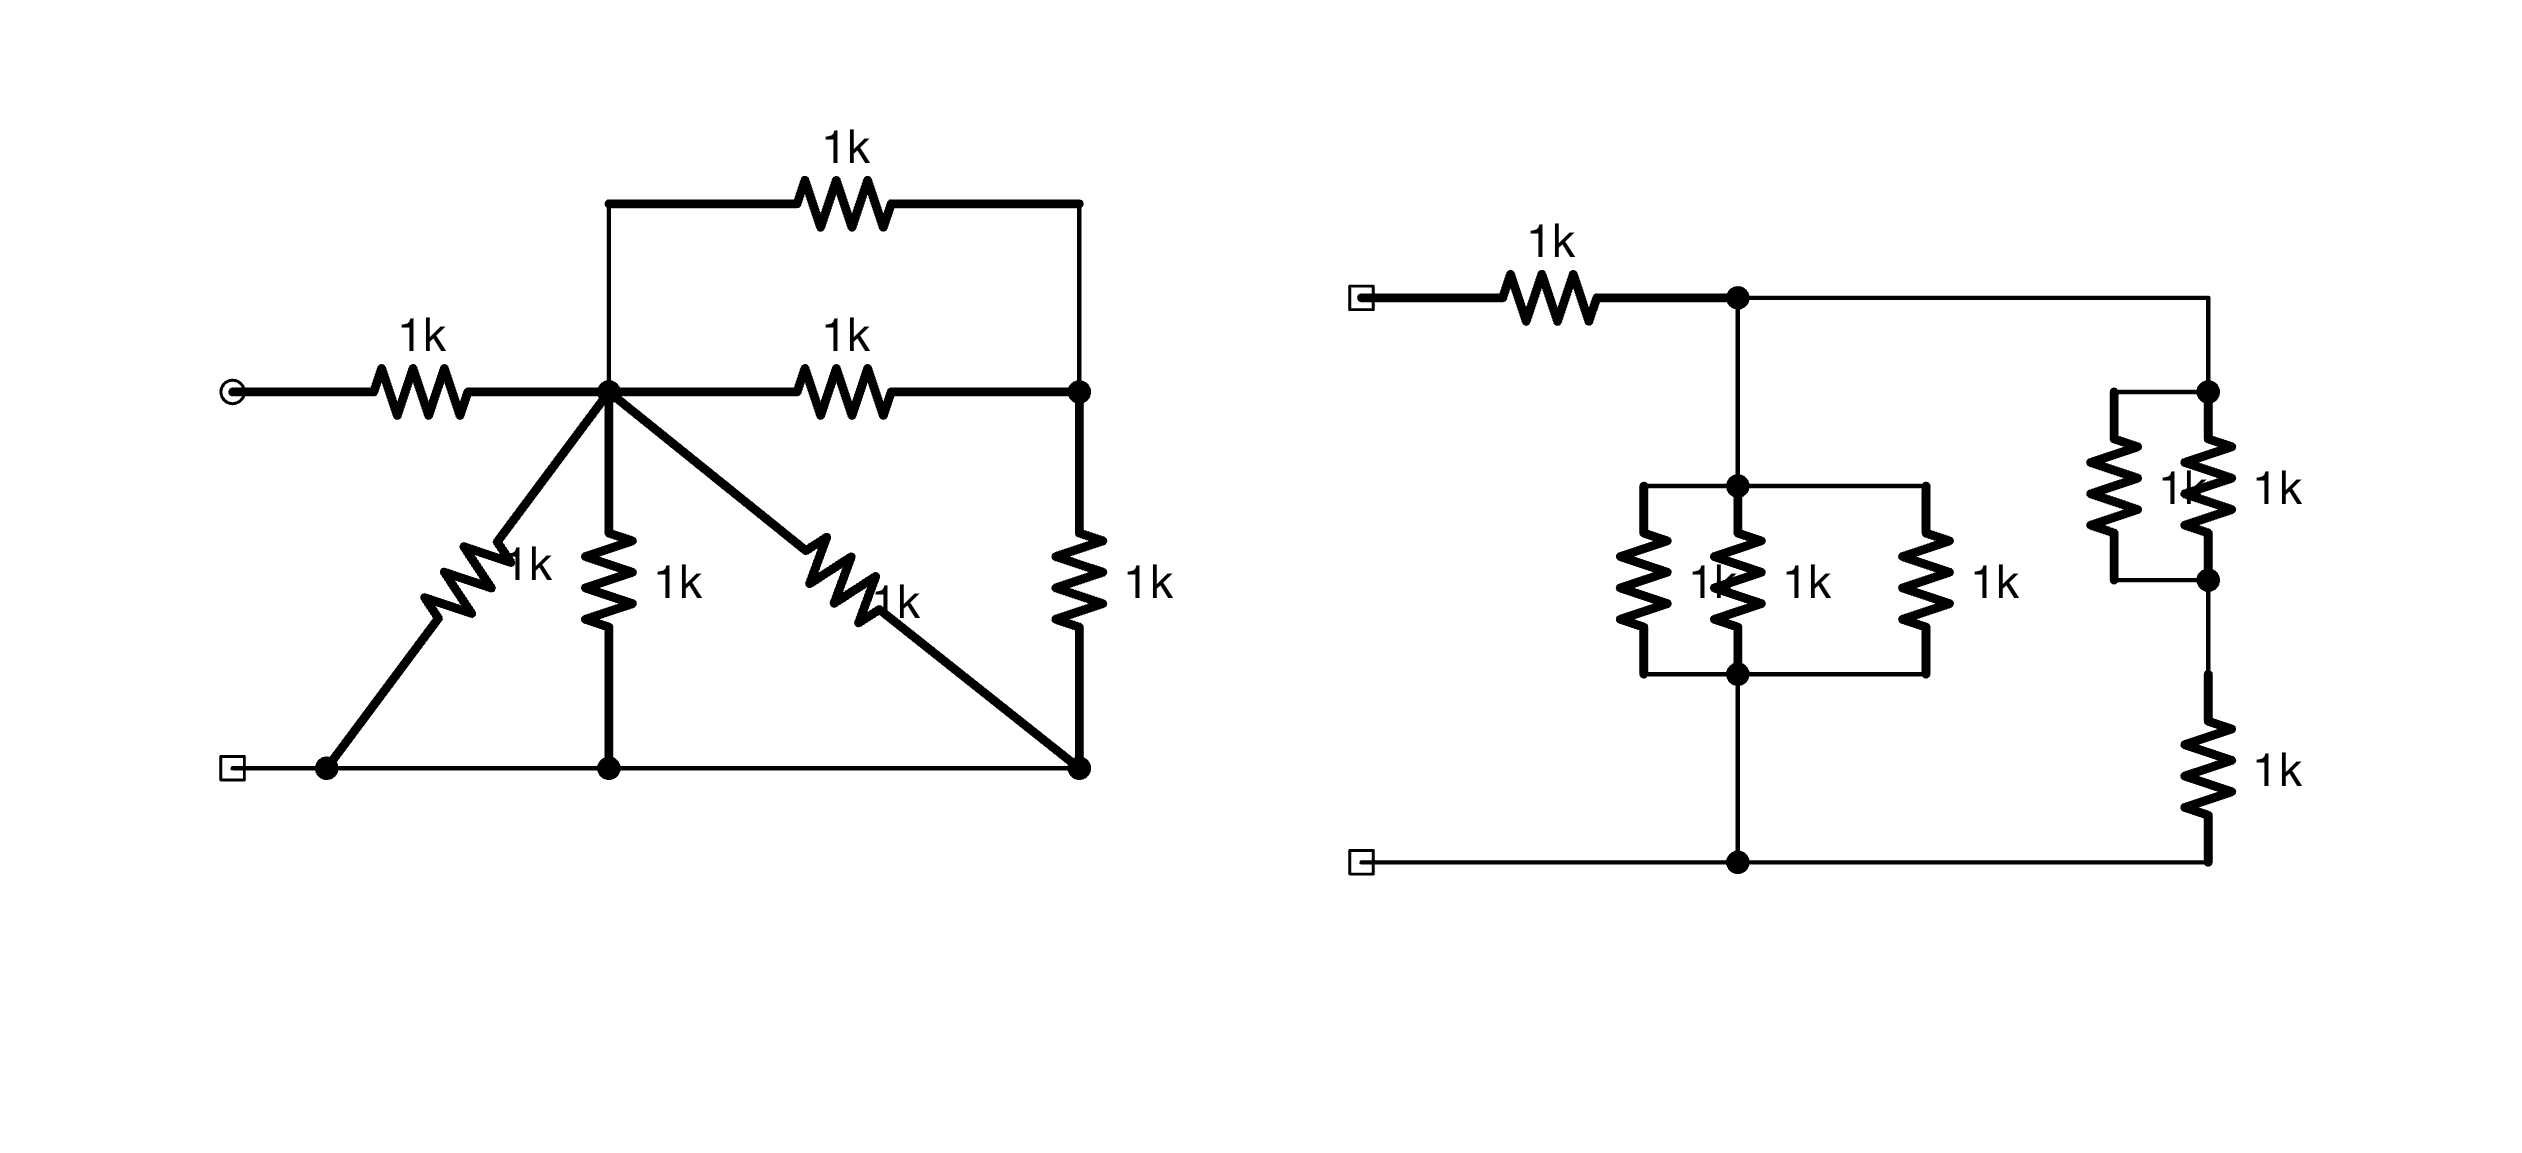
\includegraphics[width=100mm]{Image/IMG_5767AD1A8240-1.jpeg}
\end{figure}

\subsubsection{Delta to Y conversion: }
\begin{gather}
	R_A=\frac{R11\times R21}{R11+R21+R31}\\
	R_B=\frac{R31\times R21}{R11+R21+R31}\\
	R_C=\frac{R31\times R21}{R11+R21+R31}
\end{gather}
	
\begin{figure}[H]
	\centering
	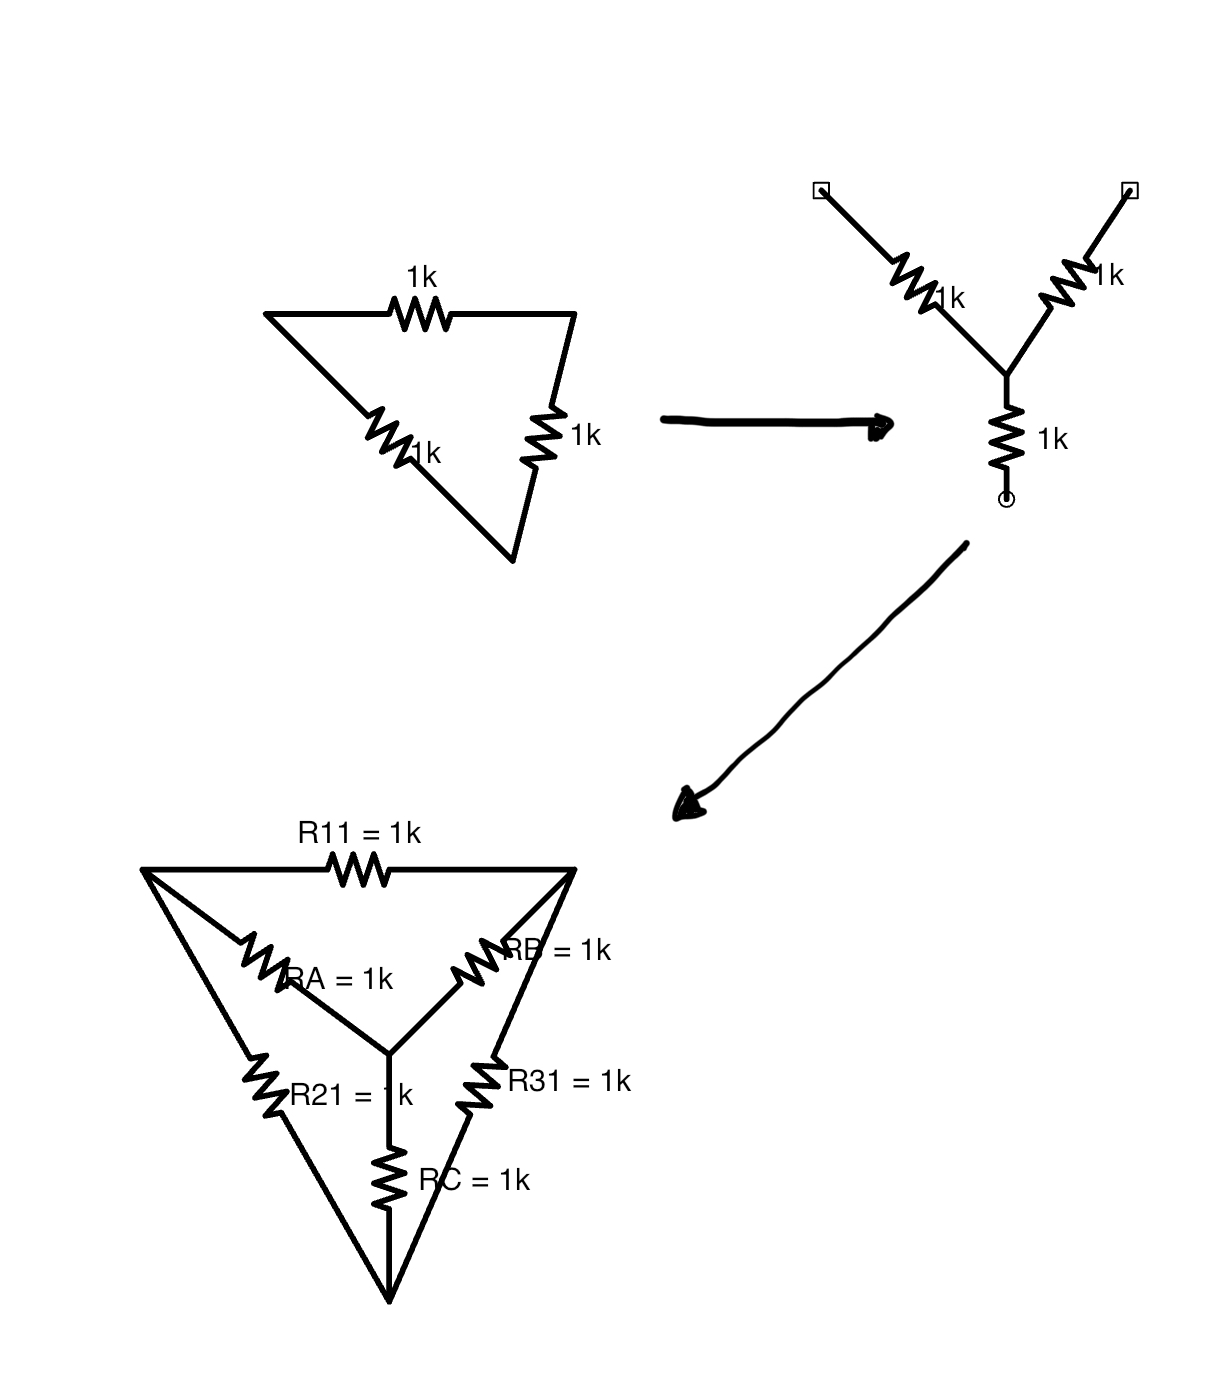
\includegraphics[width=80mm]{Image/IMG_96ACB9C21676-1.jpeg}
\end{figure}
\textbf{Example:}
\begin{figure}[H]
	\centering
	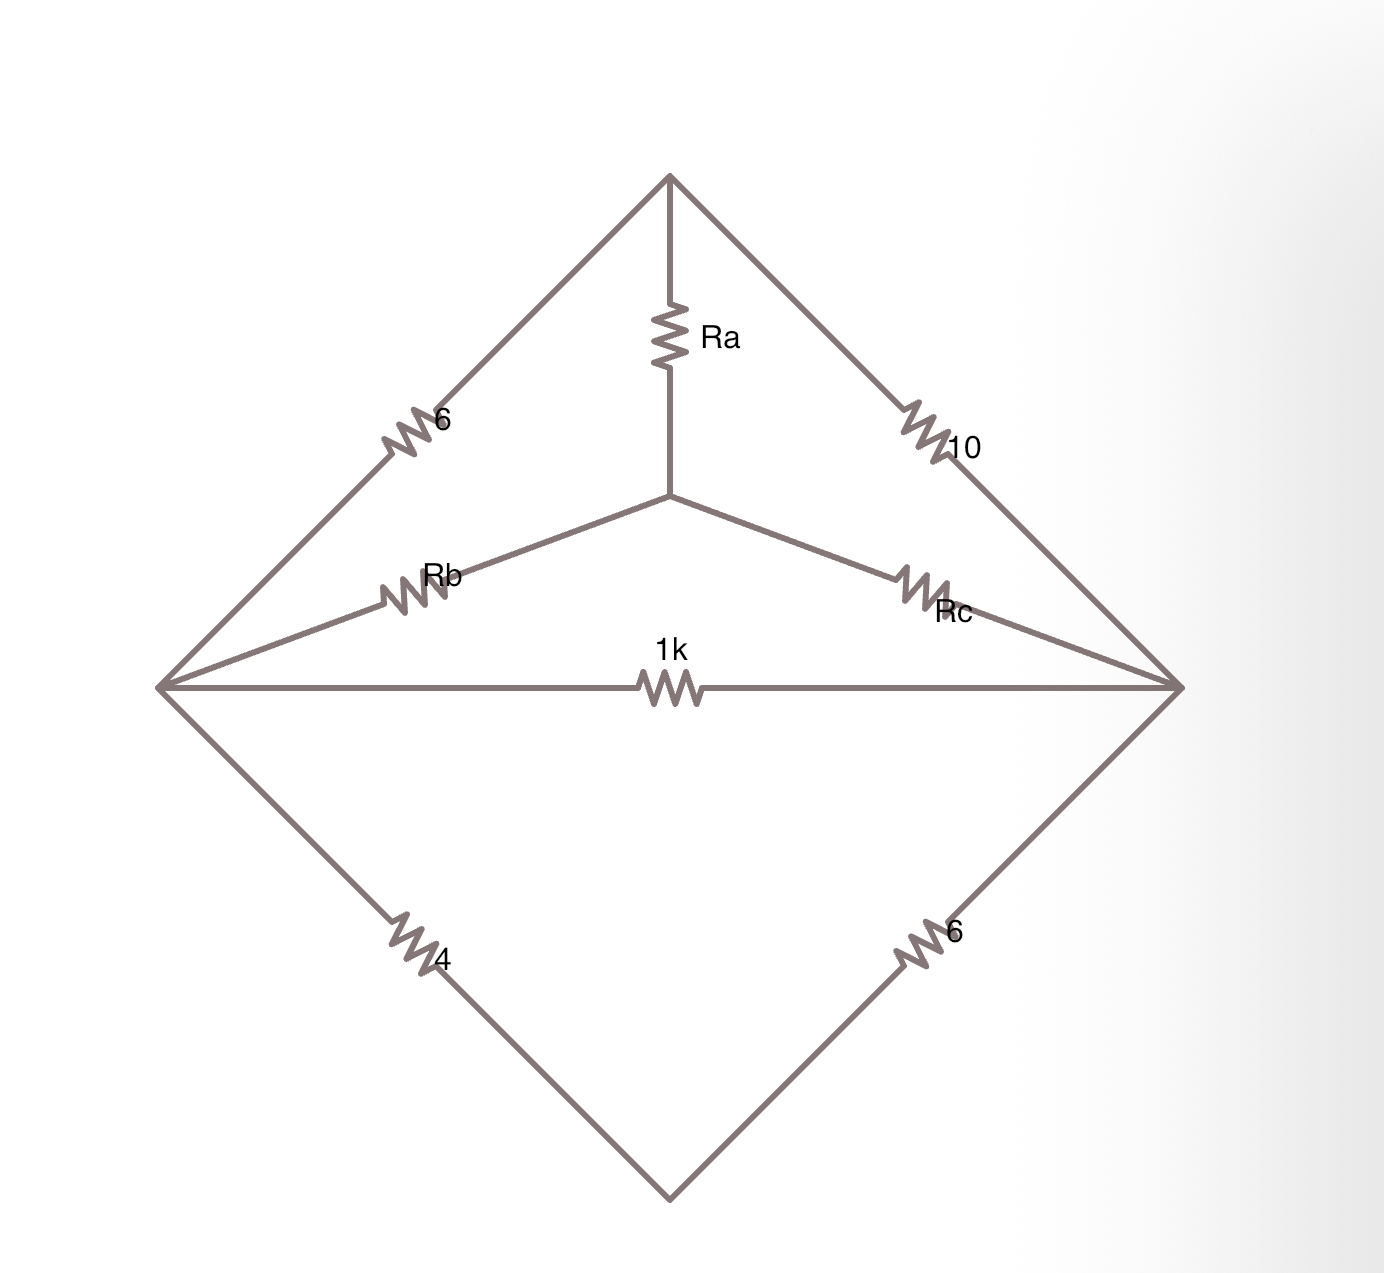
\includegraphics[width=50mm]{Image/IMG_BE86518E1F99-1.jpeg}
	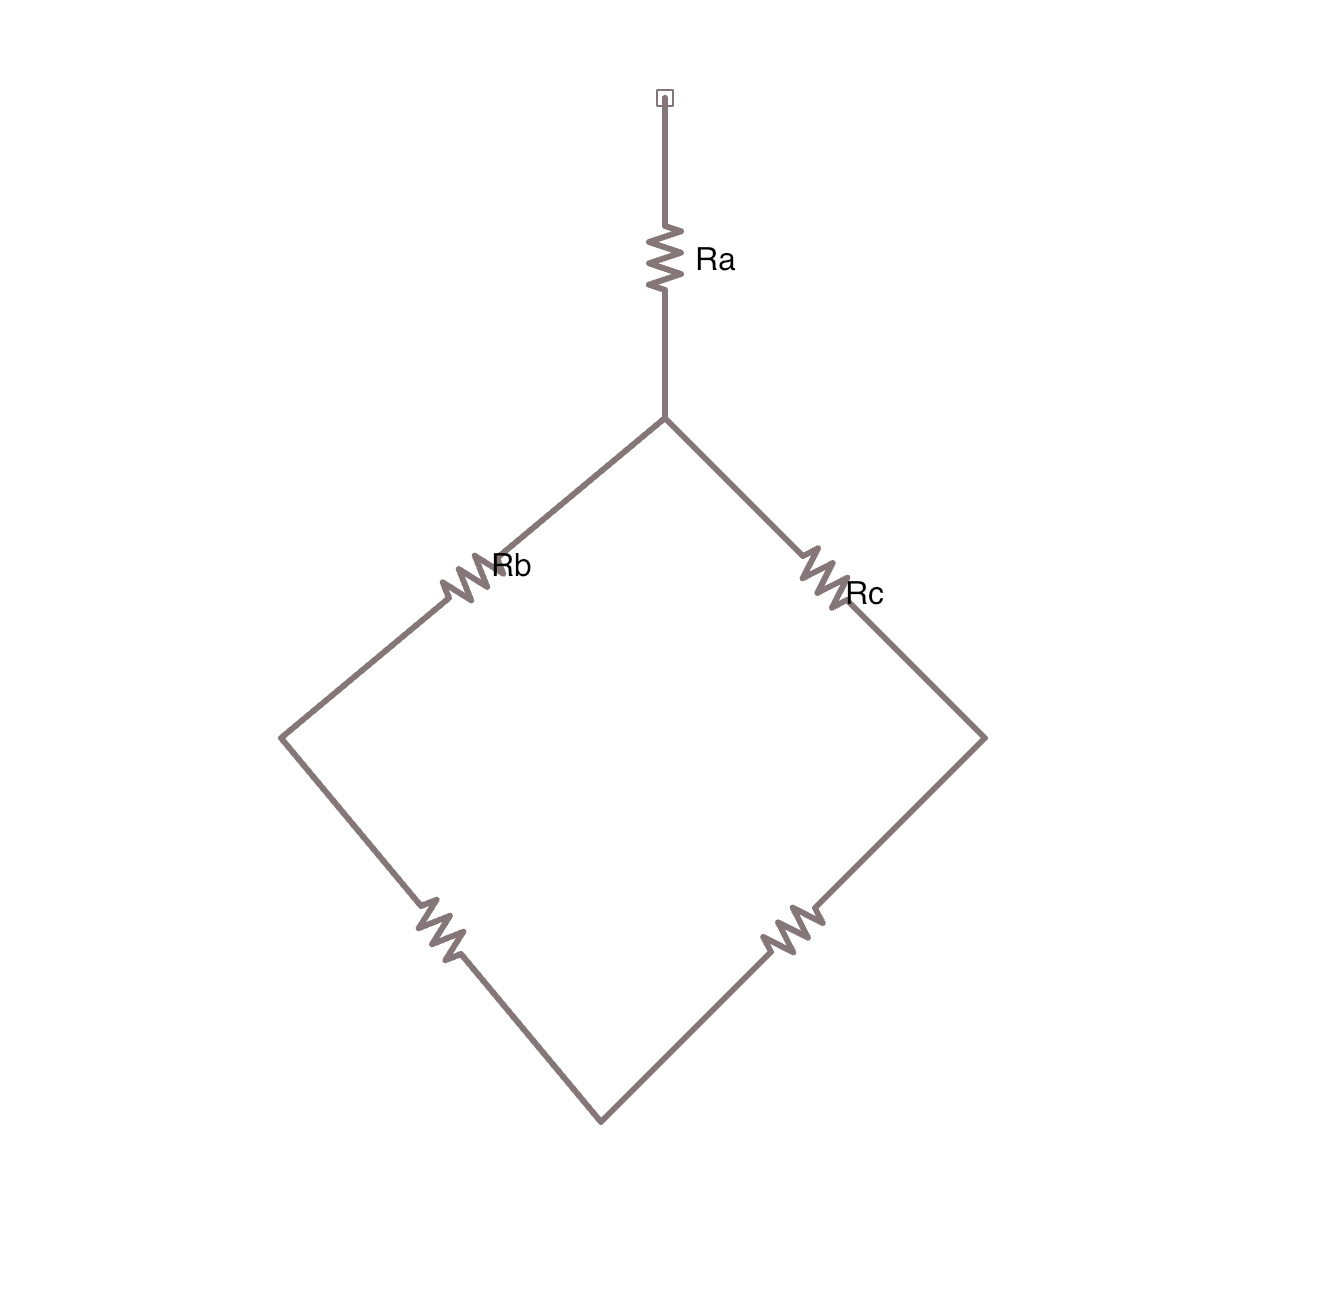
\includegraphics[width=70mm]{Image/IMG_58FAB4CBE3EB-1.jpeg}
\end{figure}
\begin{gather}
	Ra=\frac{6\times 10}{6+1+10}\\
	Rb=\frac{6\times 1}{6+1+10}\\
	Rc=\frac{1\times 10}{6+1+10}
\end{gather}
\subsection{Voltage Divider (for series circuit):}
\begin{figure}[H]
	\centering
	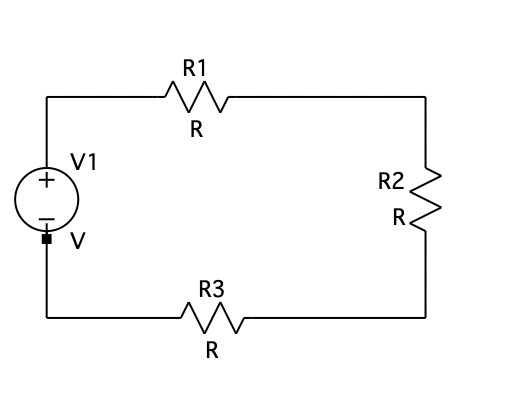
\includegraphics[width=80mm]{Image/3.jpg}
\end{figure}
\[V_{R_1}=\frac{V_s\times R_1}{R_1+R_2+R_3}\]

\subsection{Current Divider:}
\begin{figure}[H]
	\centering
	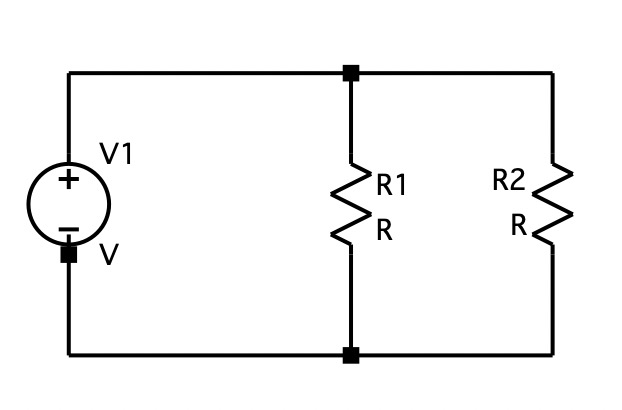
\includegraphics[width=90mm]{Image/4.jpg}
\end{figure}
\[I_{1}=\frac{I_T\times R_2}{R_1+R_2+R_3}\]\\
\[I_{2}=\frac{I_T\times R_1}{R_1+R_2+R_3}\]
\subsection{Nodal Analysis:}
\begin{enumerate}
	\item Do the KCL at nodes to get the equation.
	\item Consider all current leaving nodes except if specified.
	\item Select a reference point to compare to usually negative of the power supply or ground.
\end{enumerate}
\begin{figure}[H]
    \centering
    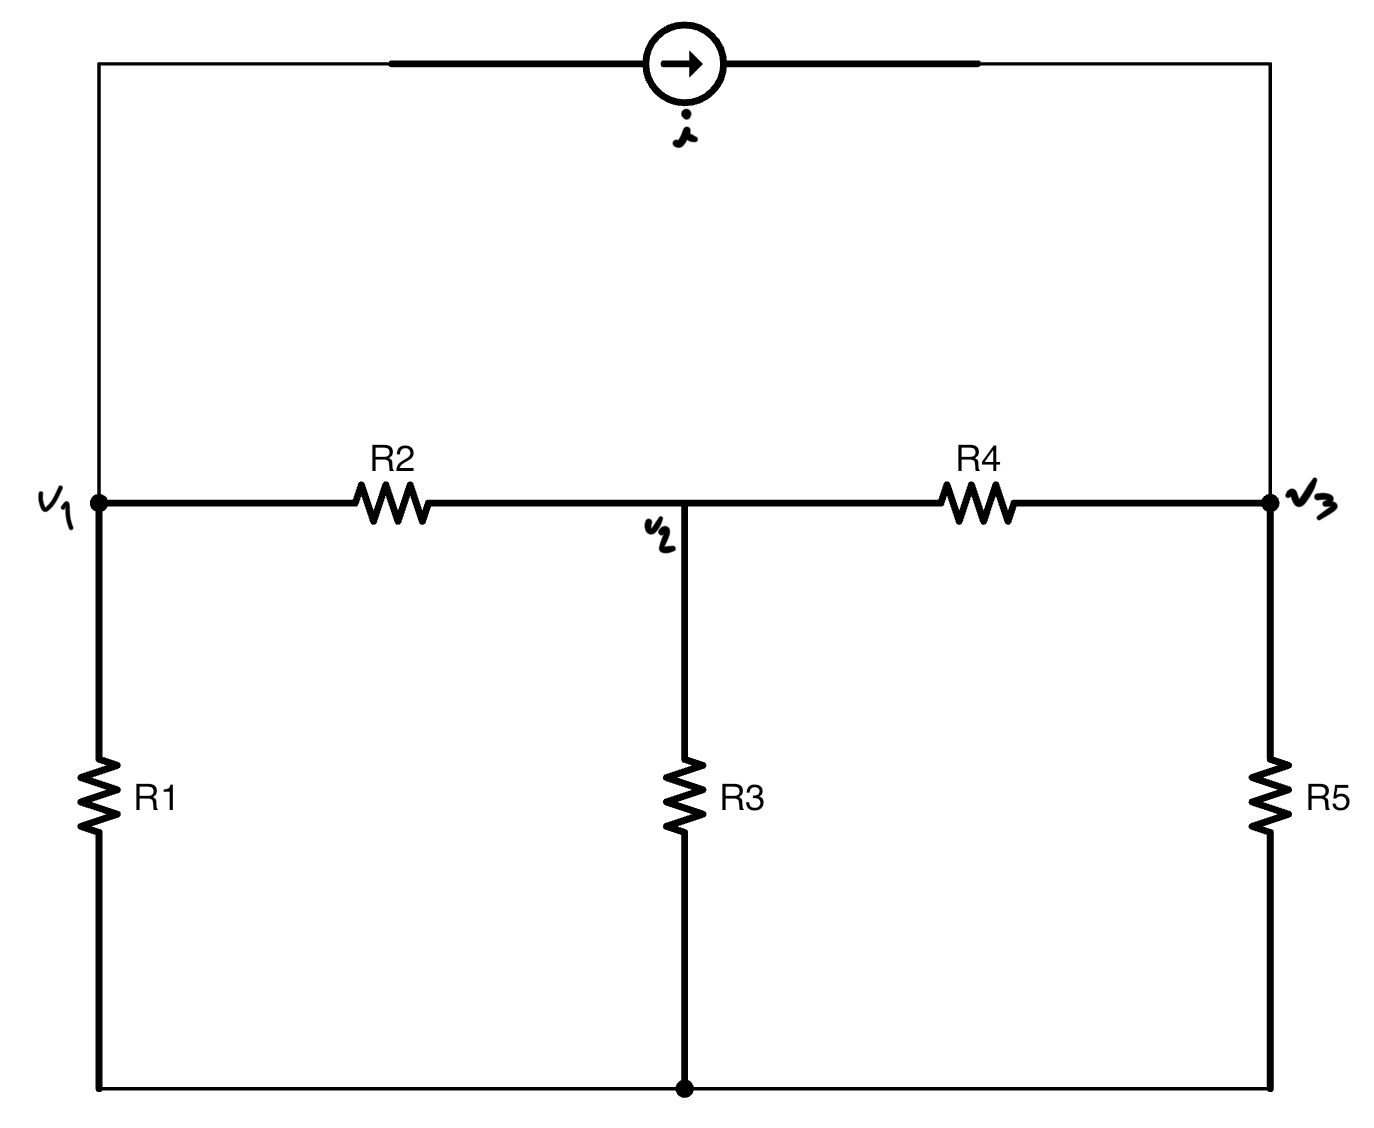
\includegraphics[width=100mm]{Image/5.jpg}
\end{figure}
\begin{gather}
    \frac{v_1-v_2}{R_2}+\frac{v_1}{R_1}+i =0\\
    \frac{v_3}{R_5}-i+\frac{v_3-v_2}{R_4} =0\\
    \frac{v_2-v_3}{R_4}+\frac{v_2-v_1}{R_2}+\frac{v_2}{R_4} =0
\end{gather}
\subsection{Node voltage with Supper Node:}
\begin{enumerate}
    \item When you have voltage source between two nodes.
    \item enclose the two nodes with dashed line positive consider that as super node.
\end{enumerate}
\begin{figure}[H]
    \centering
    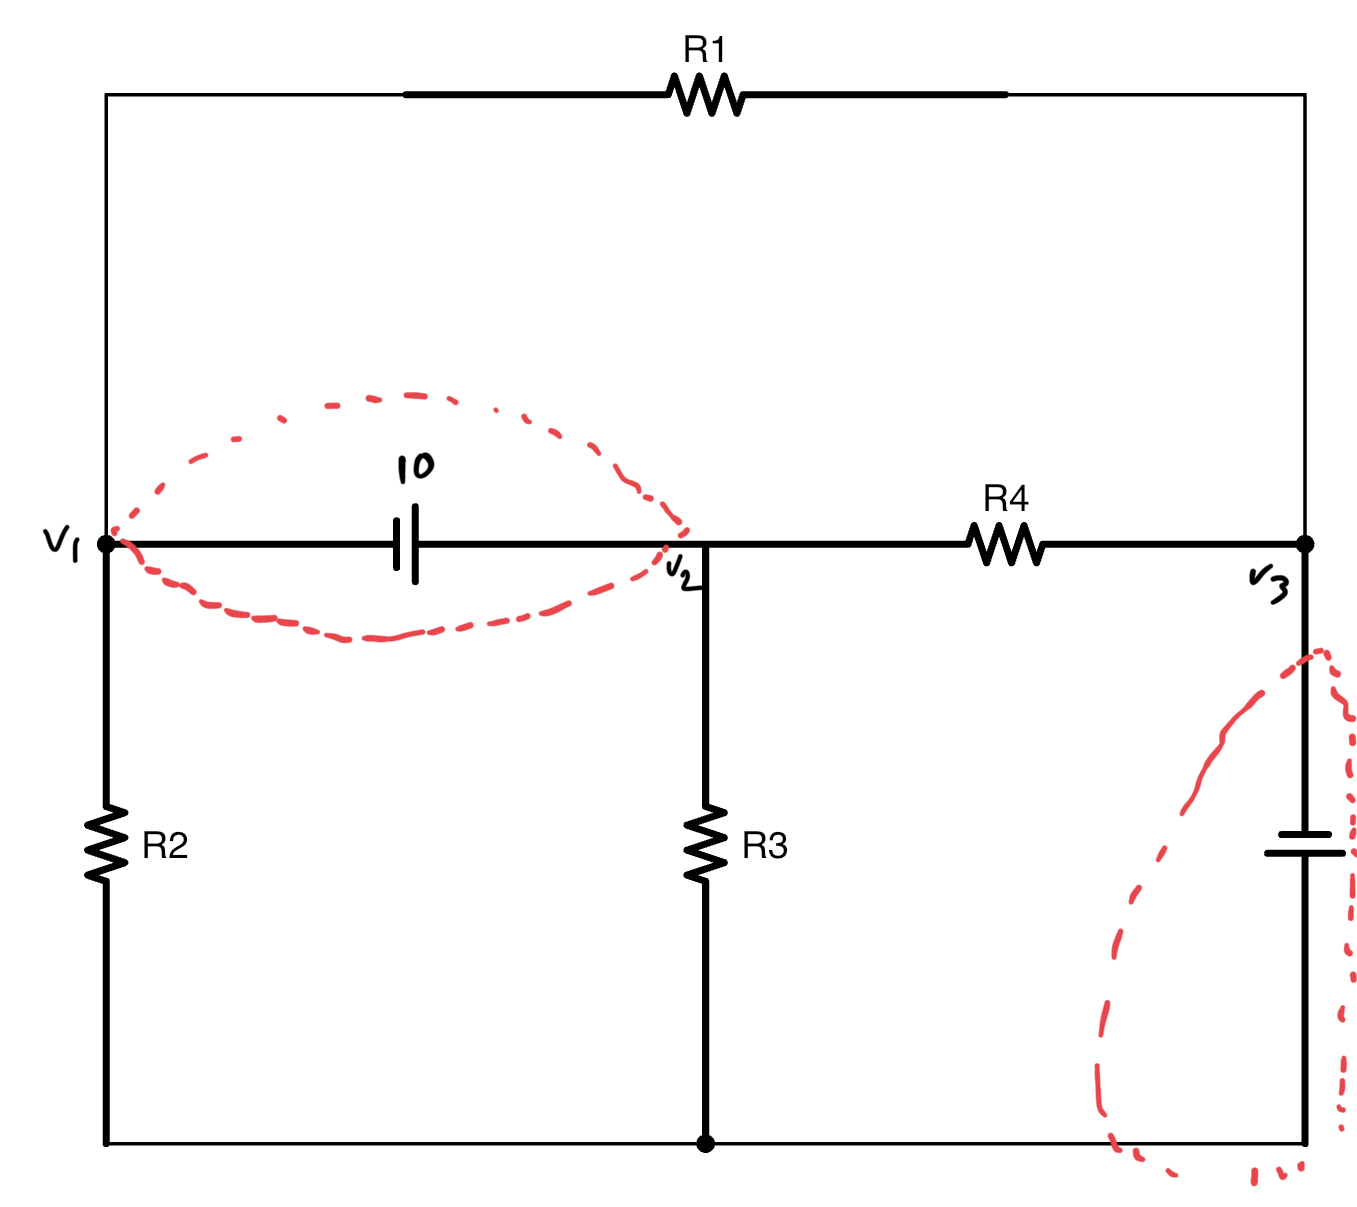
\includegraphics[width=80mm]{Image/6.jpg}
\end{figure}
\begin{gather}
    \frac{v_1}{R_2}+\frac{v_1-v_3}{R_1}+\frac{v_2}{R_4}+\frac{v_2-v_3}{R_3}=0\\
    kvl\rightarrow v1-10+v_2=0
\end{gather}
\subsection{Node Voltage Analysis with Controlled Source:}

\begin{figure}[H]
    \centering
    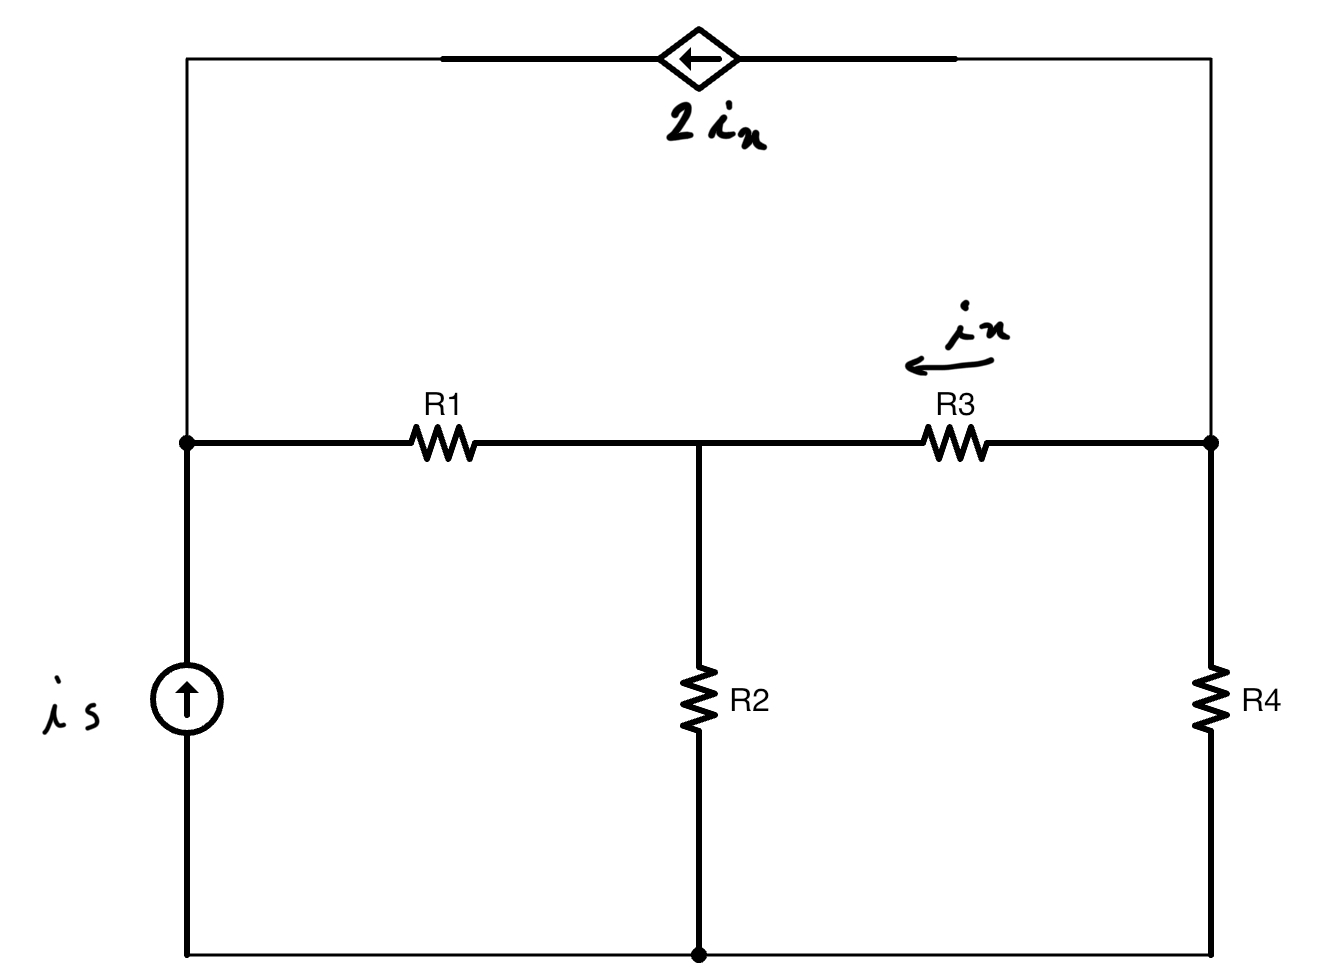
\includegraphics[width=90mm]{Image/8.jpg}
\end{figure}
\begin{align}
    -i_s-2i_x+\frac{v_1-v_2}{R_1}=0\\
    \frac{v_2}{R_2}+\frac{v_2-v_1}{R_1}-i_x=0\\
    v_x+\frac{v_3}{R_4}+2i_x=0\\
    i_x=\frac{v_3-v_2}{R_3}
\end{align}
\subsection{Mesh Current Analysis:}
\begin{enumerate}
    \item Assume loop current direction(clockwise)
    \item Current going to source from \textbf{negative} to \textbf{positive} is negative volt
    \item Current going in load or Resistor results, in positive; neighboring current goes negative
\end{enumerate}
\begin{figure}[H]
    \centering
    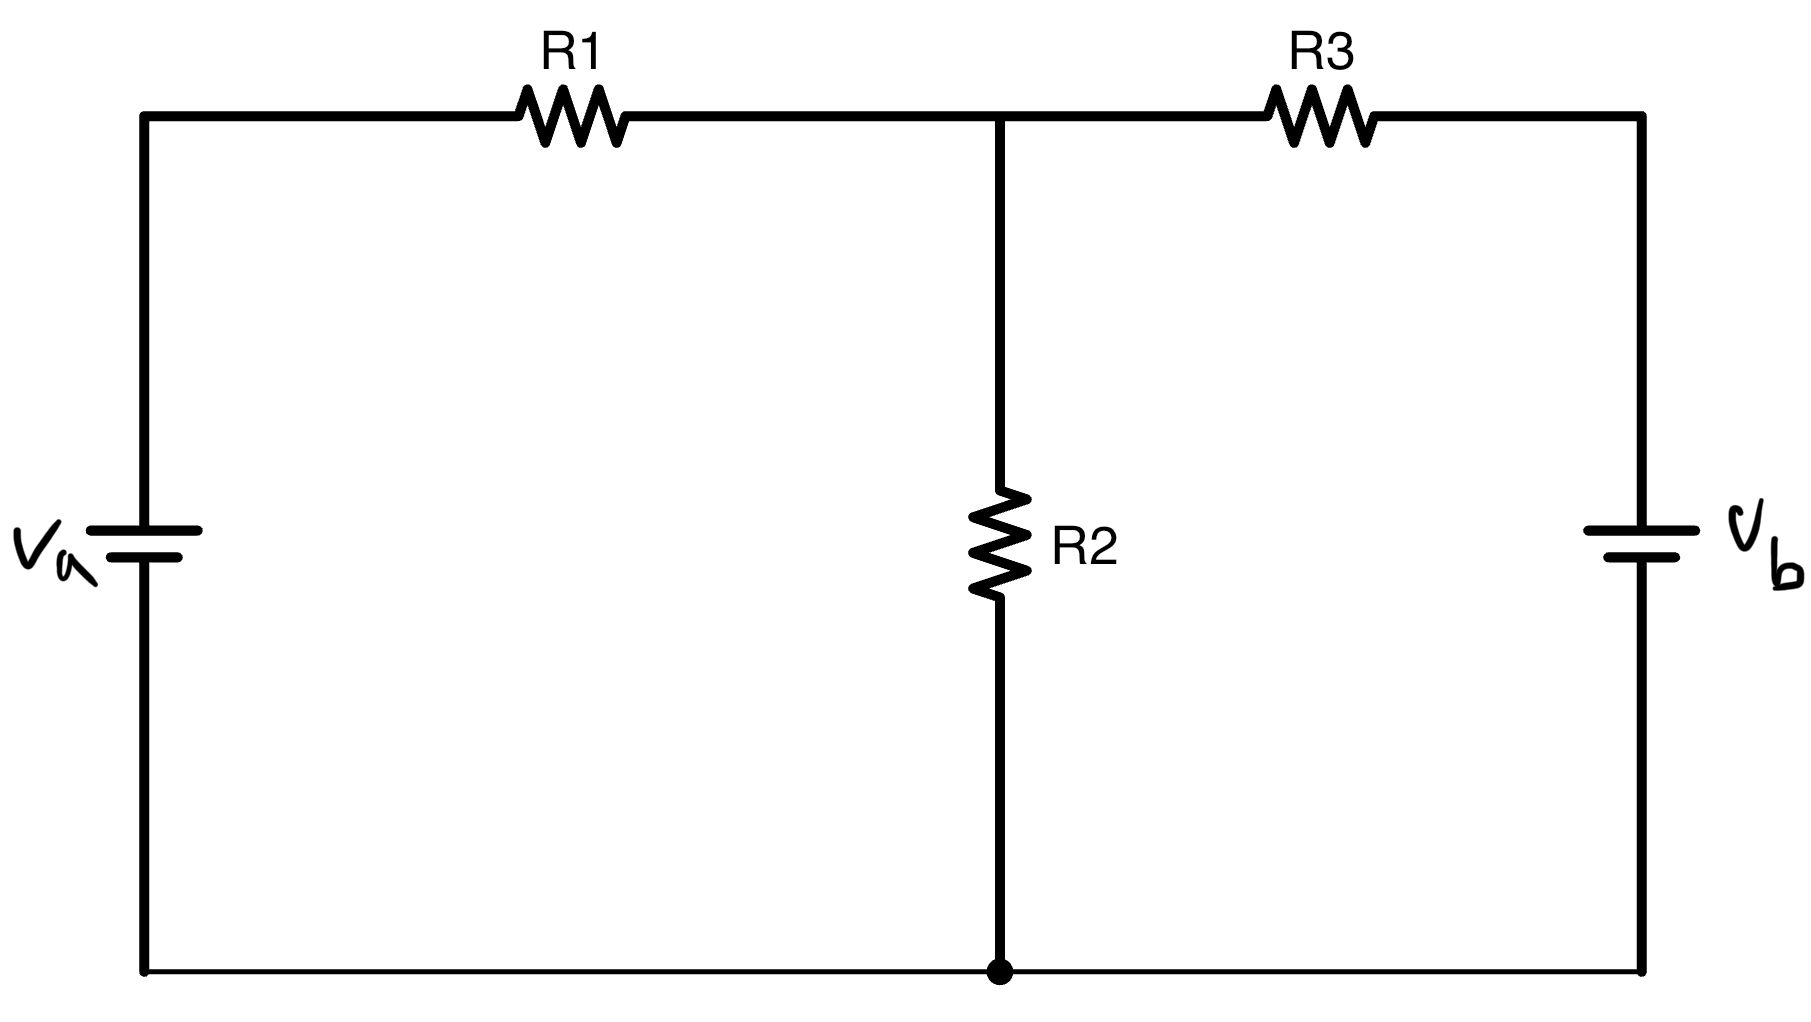
\includegraphics[width=90mm]{Image/9.jpg}
\end{figure}
\begin{align}
    -v_a+i_1R_1+(i_1-i_2)R_2=0\\
    v_b+(i_2-i_1)R_2+i_2R_3=0
\end{align}
\subsection{Mesh Current Analysis with Shared Current Source Between Loops:(Supper Mesh) }
Treat the two loops with current source as one supper mesh.
\begin{figure}[H]
    \centering
    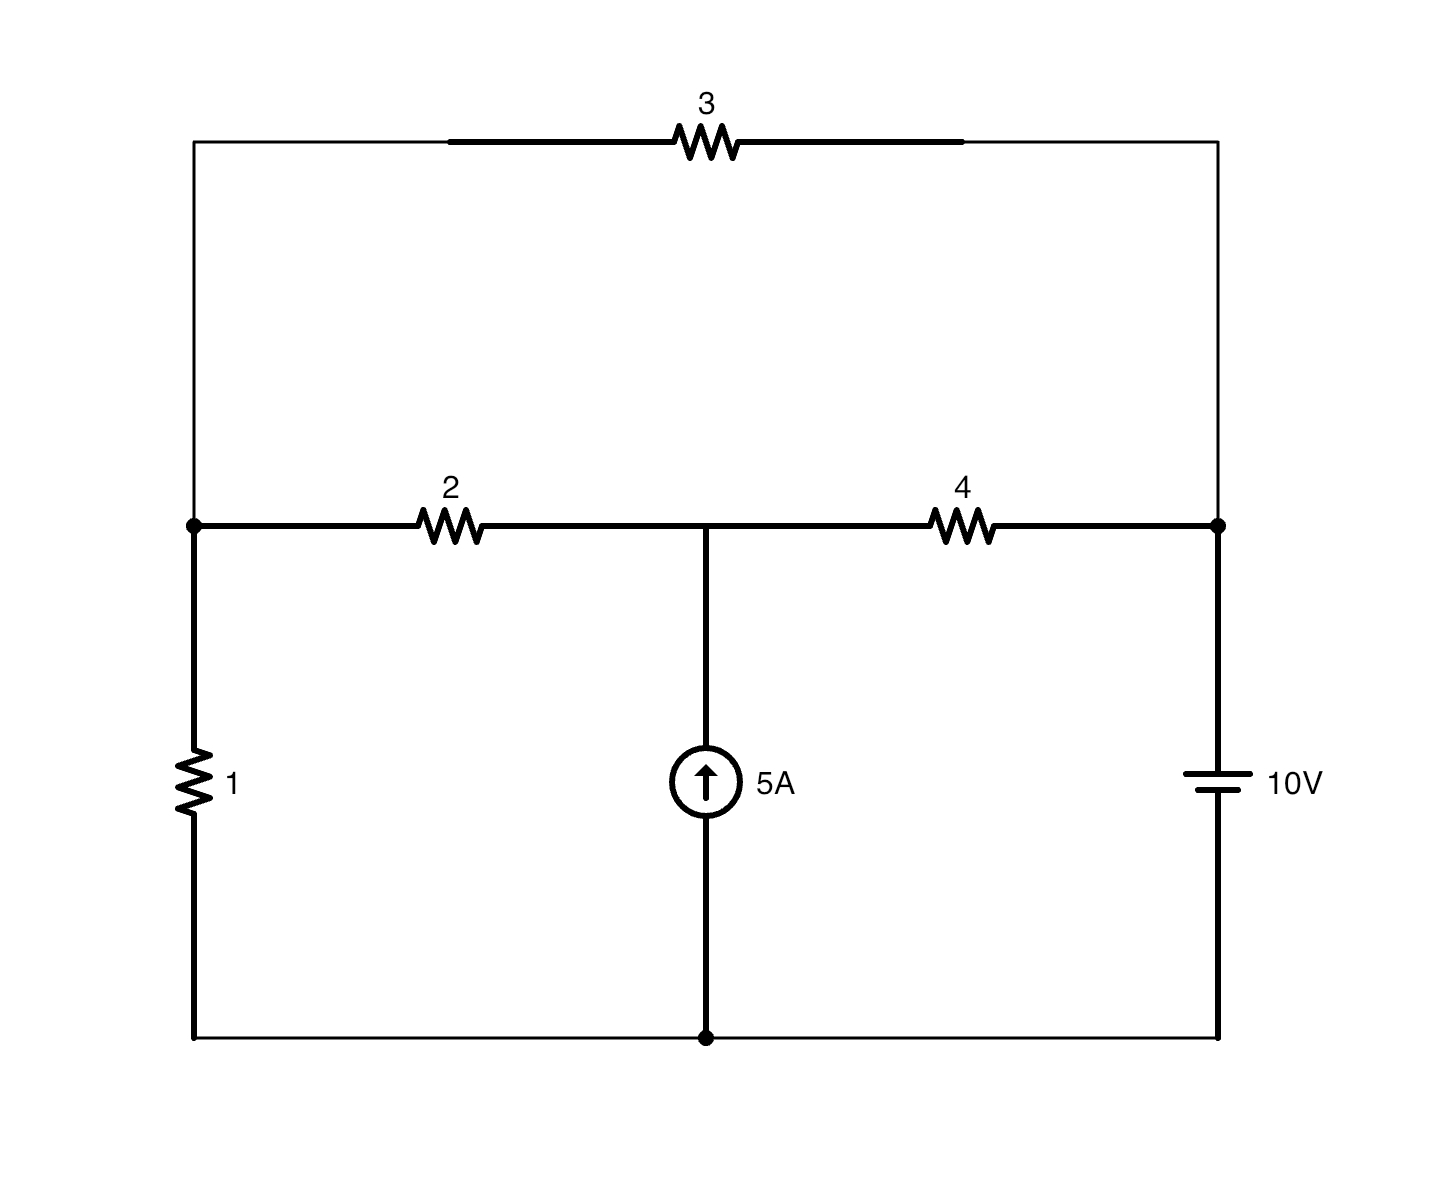
\includegraphics[width=100mm]{Image/10.jpg}
\end{figure}
KVL for supper mesh 1,2
\begin{align}
    i_11\Omega+(i_1-i_3)2\Omega+(i_2-i_3)4\Omega+10v=0\\
    (i_3-i_1)2\Omega+i_3 3\Omega +(i_3-i_2)4\Omega=0\\
    i_2-i_1=5A 
\end{align}
\subsection{Mesh Current Analysis with Controlled Source:}
\begin{figure}[H]
    \centering
    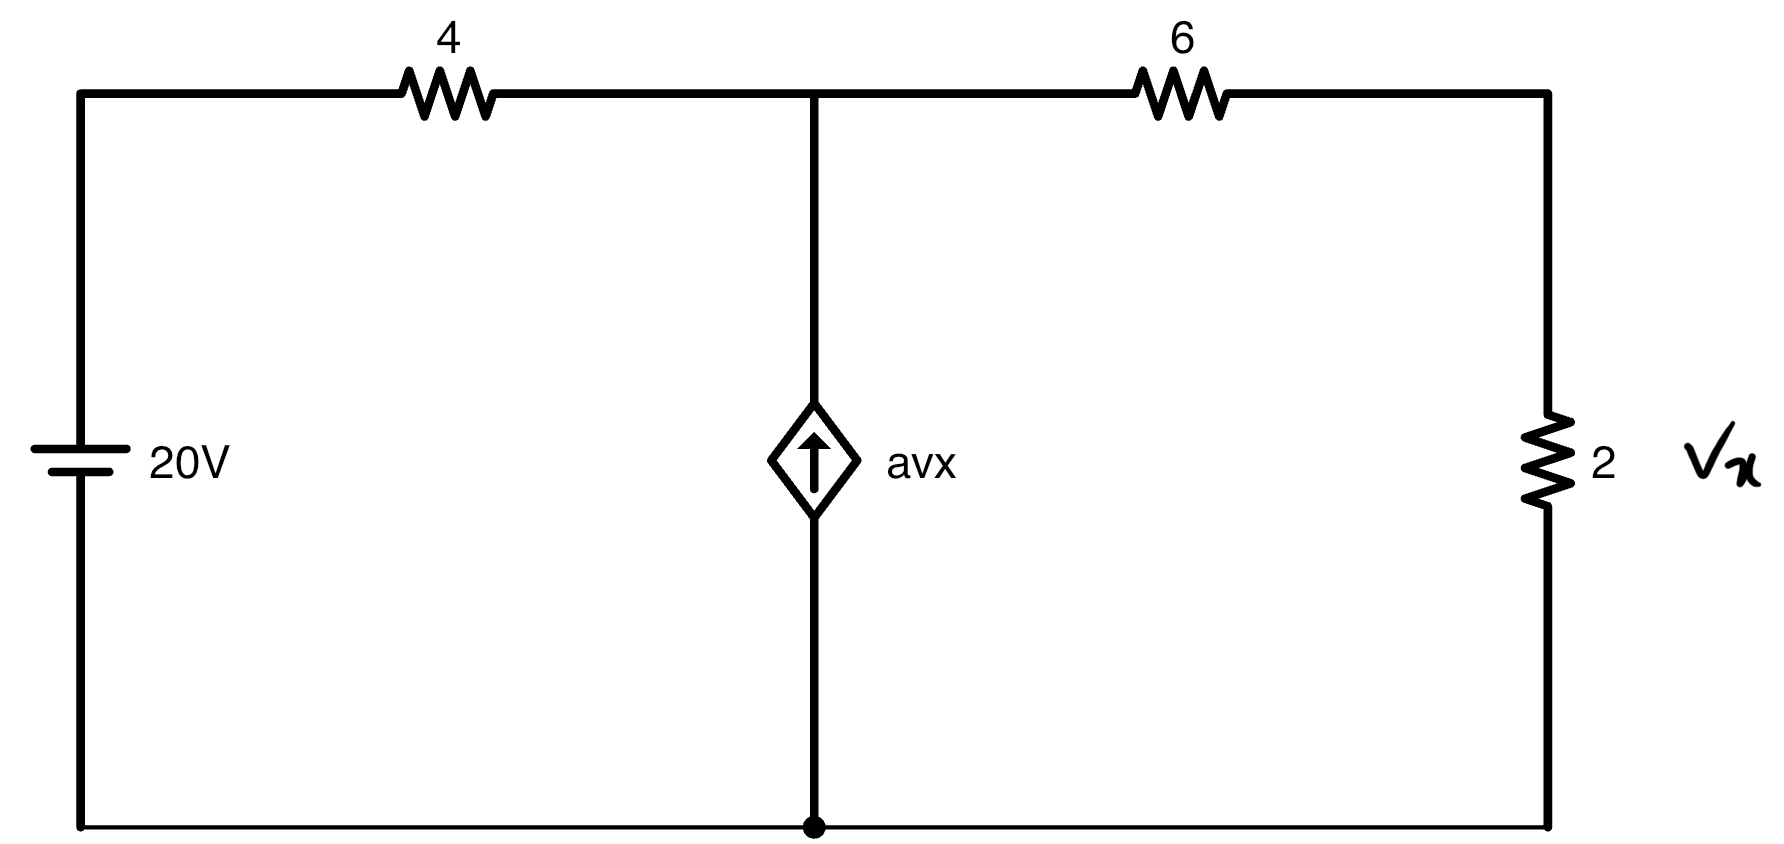
\includegraphics[width=90mm]{Image/11.jpg}
\end{figure}
\begin{align}
    V_x &=i_2 2\Omega\\
    i_2-i_1 &=aV_x\\
    -20+i_14\Omega+i_26\Omega+i_22\Omega &=0\\
    i_2-i_1 &=a(i_2\times 2\Omega)\\
    i_1 &=1A\\
    i_2 &=2A
\end{align}
\subsection{Thevenin Equivalent Circuit:}
Any circuit can be reduced to voltage source $V_{oc}$ or $V_{TH}$ and a series resistor to $R_{TH}$. $V_{oc}$=open circuit voltage.\\
\textbf{Steps:}
\begin{enumerate}
    \item\underline{ To find $R_{TH}$} Remove current sources and short voltage sources
    \item \underline{To find $V_{TH}$} Remove $R_L$ and find v across open
   % \item Open circuit and point of intended load. Calculate open circuit voltage $v_{oc}=v_{TH}$
   % \item Short all voltage sources open all current sources find $R_{TH}$ or find $I_{R_{TH}}$(short circuit current).
    \[R_{TH}=\frac{v_{oc}}{I_{sc}}\]
\end{enumerate}
\textbf{Example:}
\begin{figure}[H]
    \centering
    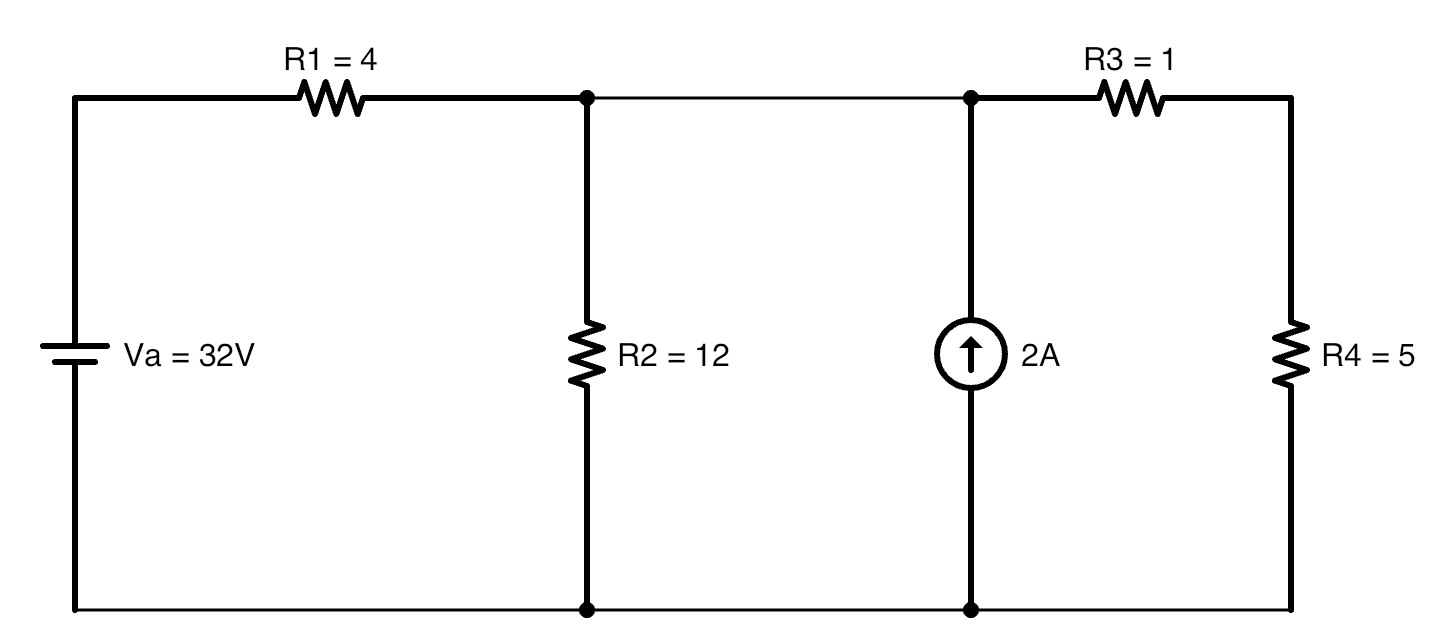
\includegraphics[width=100mm]{Image/12.jpg}
    \end{figure}
    First step:
    \begin{figure}[H]
    \centering
    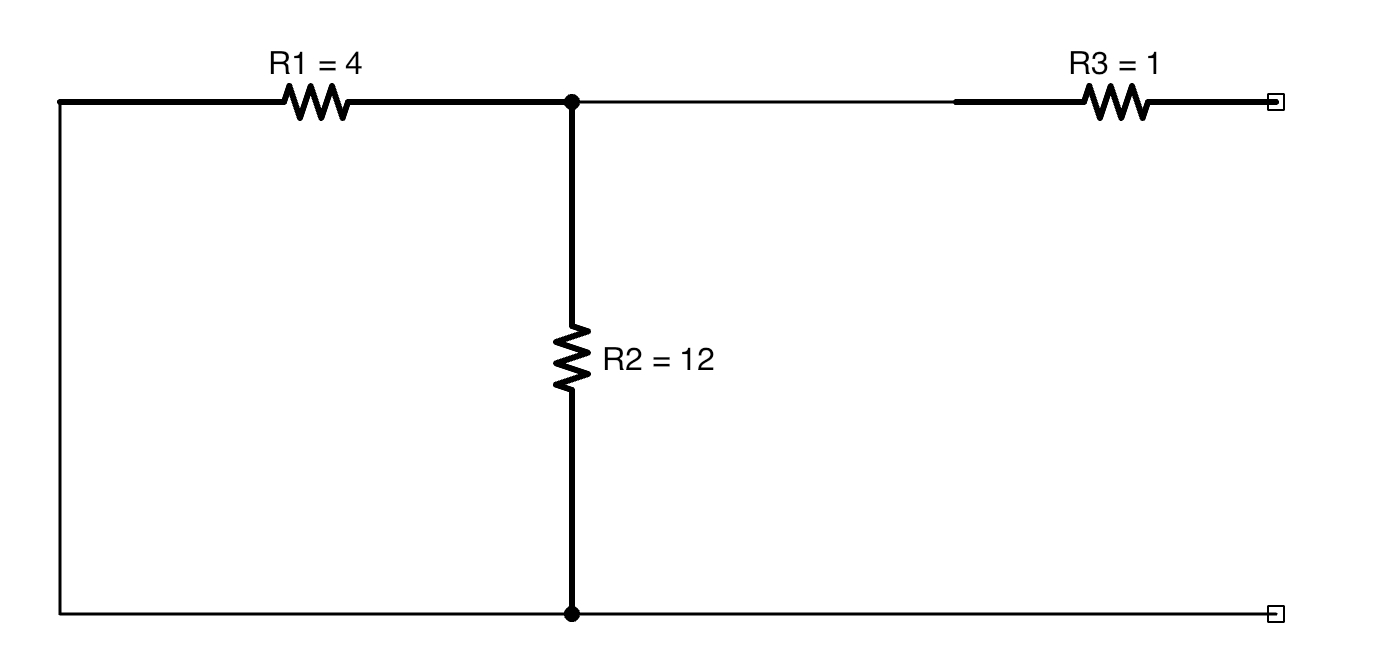
\includegraphics[width=100mm]{Image/14.jpg}
    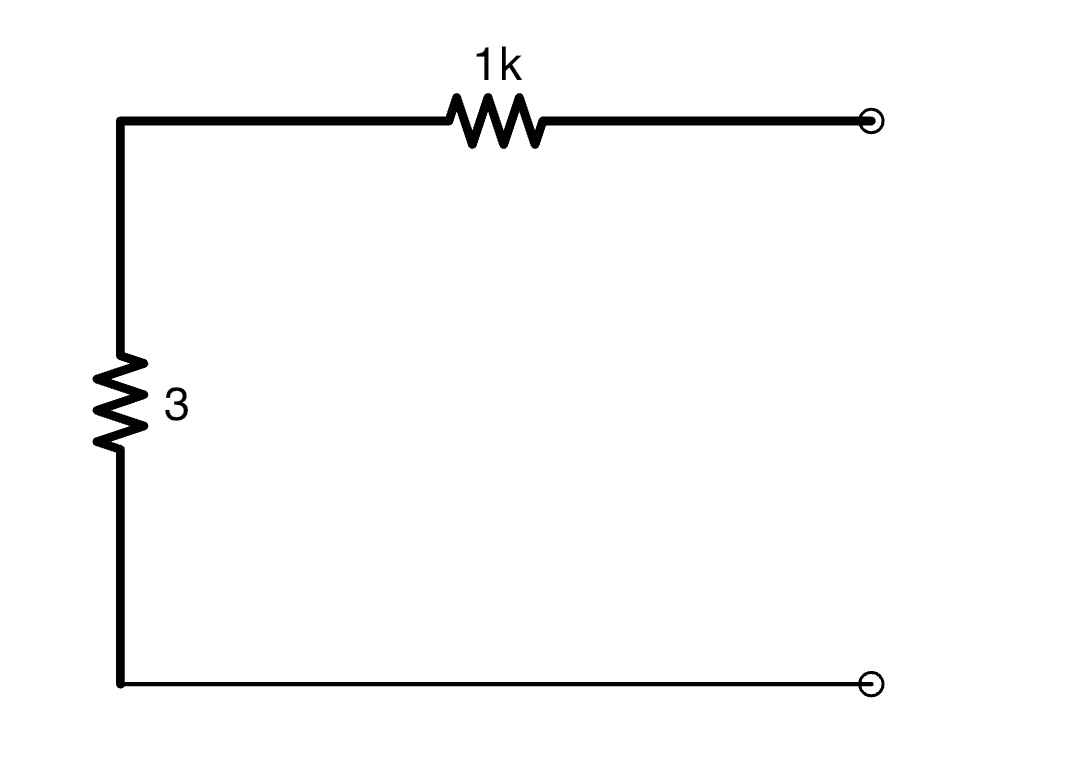
\includegraphics[width=80mm]{Image/15.jpg}
    \[R_{TH}=4\Omega\]
\end{figure}
Step two:
\begin{figure}[H]
    \centering
    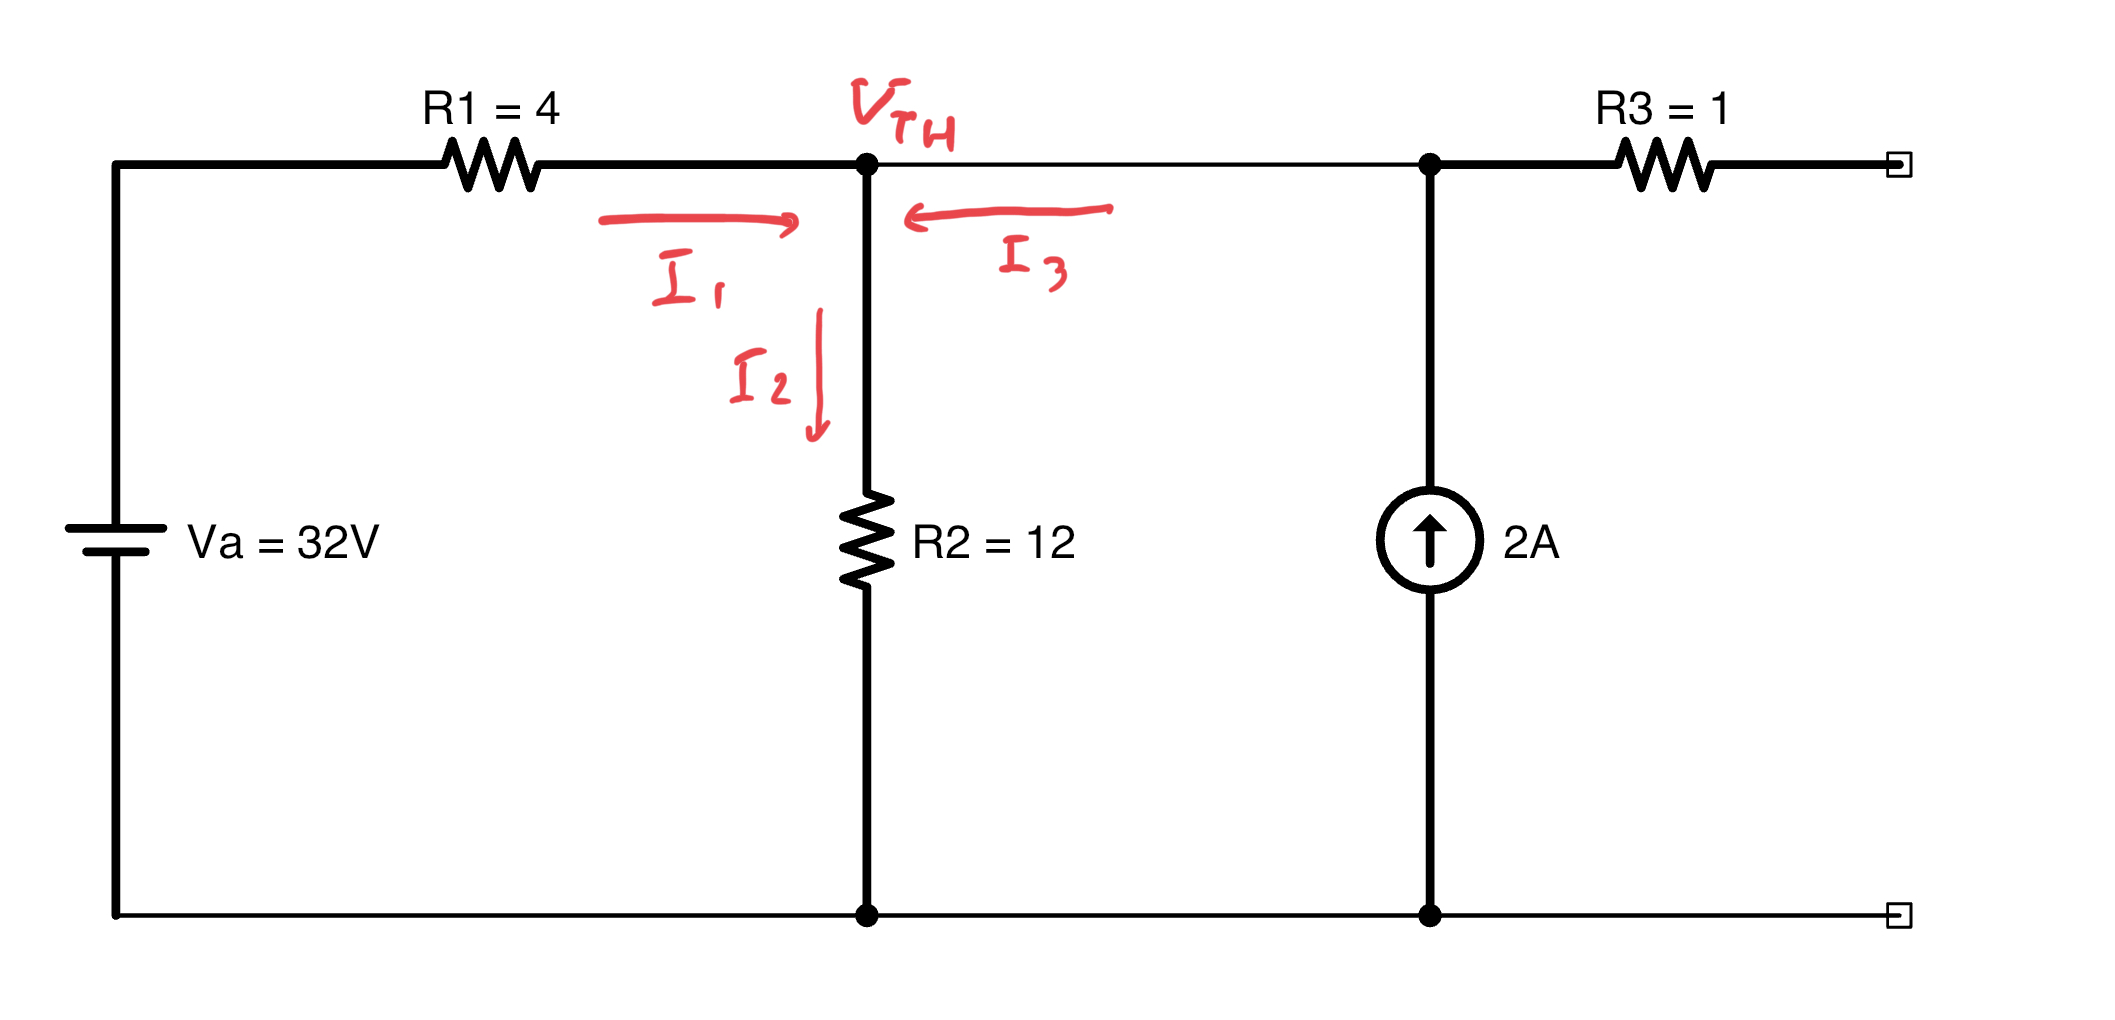
\includegraphics[width=100mm]{Image/16.jpg}
\end{figure}
\begin{gather}
    I_1+I_3=I_2\\
    \frac{32-V_{TH}}{4}+2=\frac{V_{TH}}{12}\\
    94-3V_{TH}+24=V_{TH}\\
    120=4V_{TH}\\
    V_{TH}=\frac{120}{4}=30V
\end{gather}
\begin{figure}[H]
    \centering
    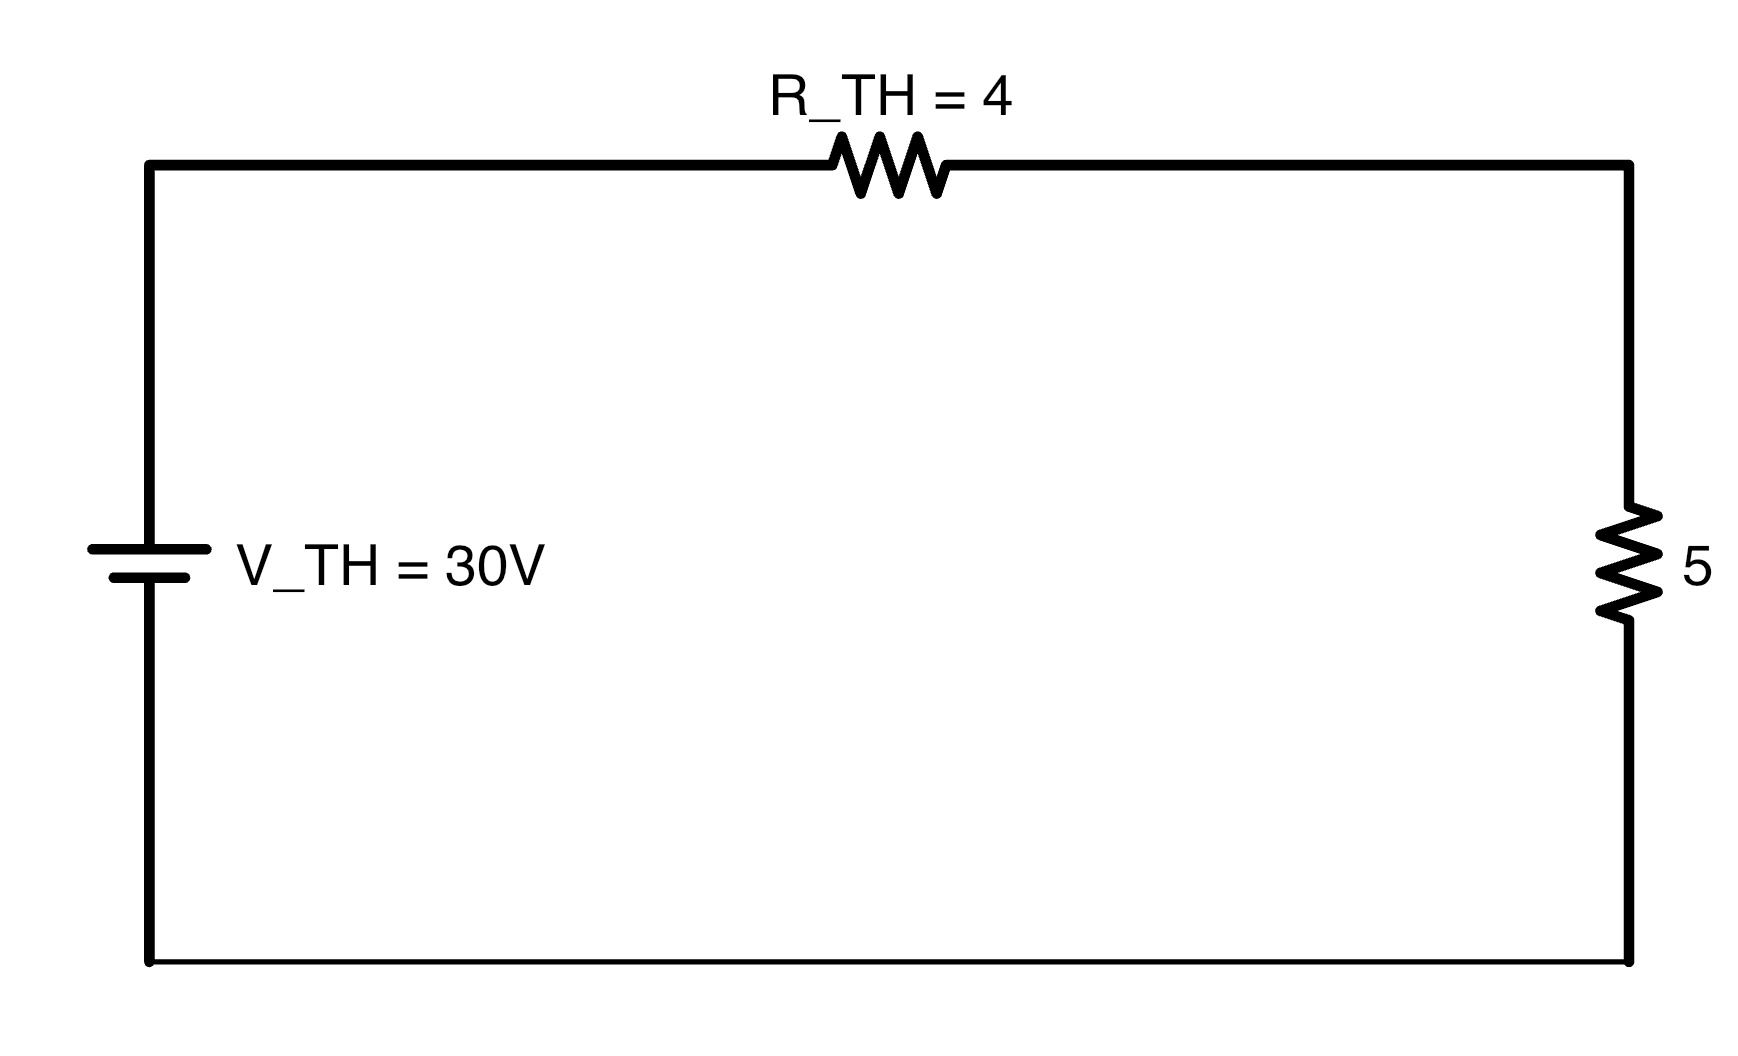
\includegraphics[width=90mm]{Image/17.jpg}
\end{figure}
\[I=\frac{V}{R_{TH}}=\frac{30V}{(4+5)\Omega}=33.3\]
\subsection{Norton's Theorem:}
\begin{enumerate}
    \item determine $V_{OC}=V_{TH}$. Determine short circuit $I_{SC}=I_{IN}$. Zero the independent source and find $R_{TH}$(Do not zero of the dependent sources)
    \item Use the equation $V_{TH}=R_{TH}I_N$
    \item Thevenin equivalent consist of $V_{TH}$  in $R_{TH}$. Norton equivalent $I_{SC}$parallel with $R_{TH}$
\end{enumerate}
\begin{figure}[H]
    \centering
    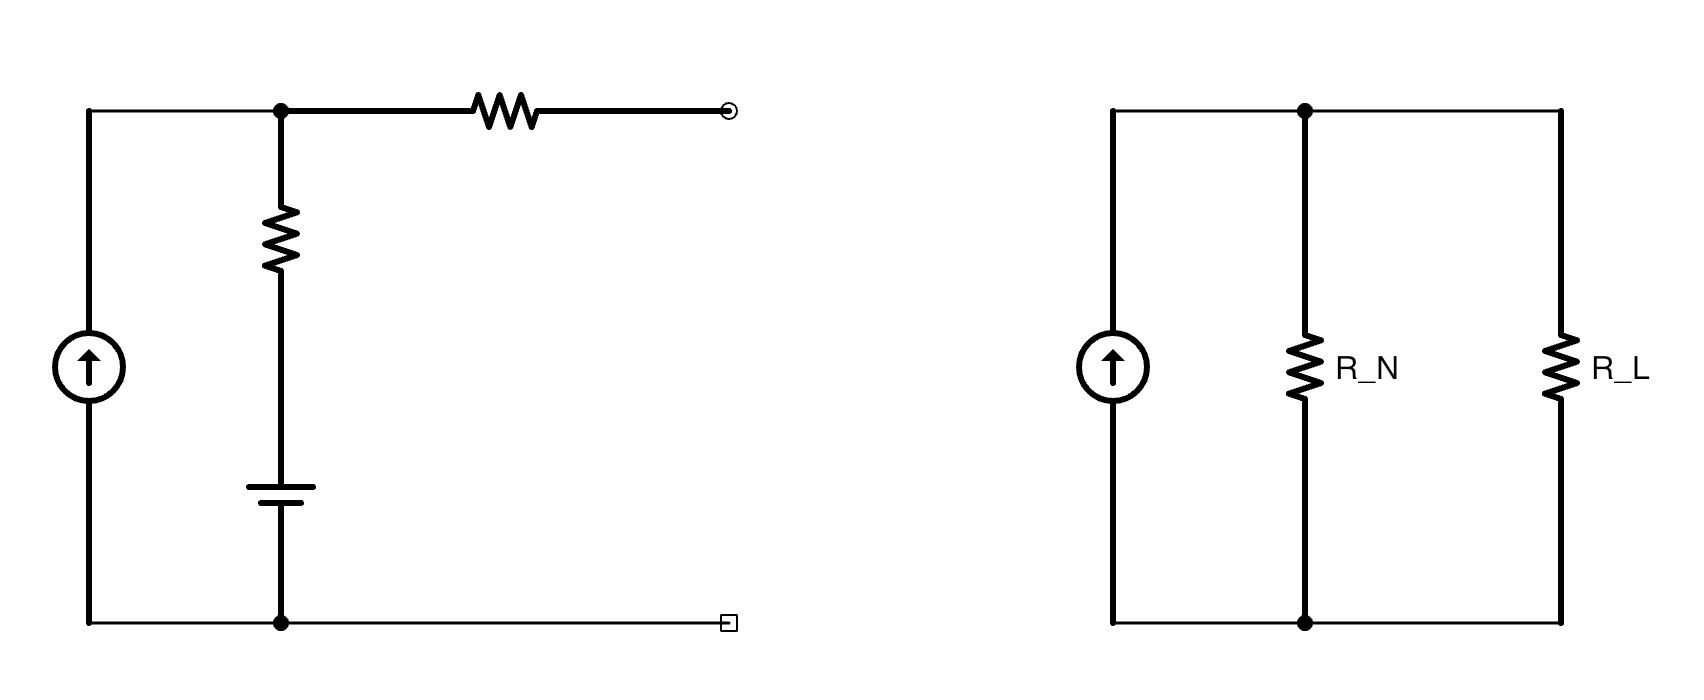
\includegraphics[width=130mm]{Image/18.jpg}
\end{figure}
\[R_N=R_{TH}\]
\[I_L=I_N(\frac{R_N}{R_N+R_L})\]
\[I_N=\frac{V_{TH}}{R_{TH}}=\frac{V_{TH}}{ER_N}\]
\begin{figure}[H]
    \centering
    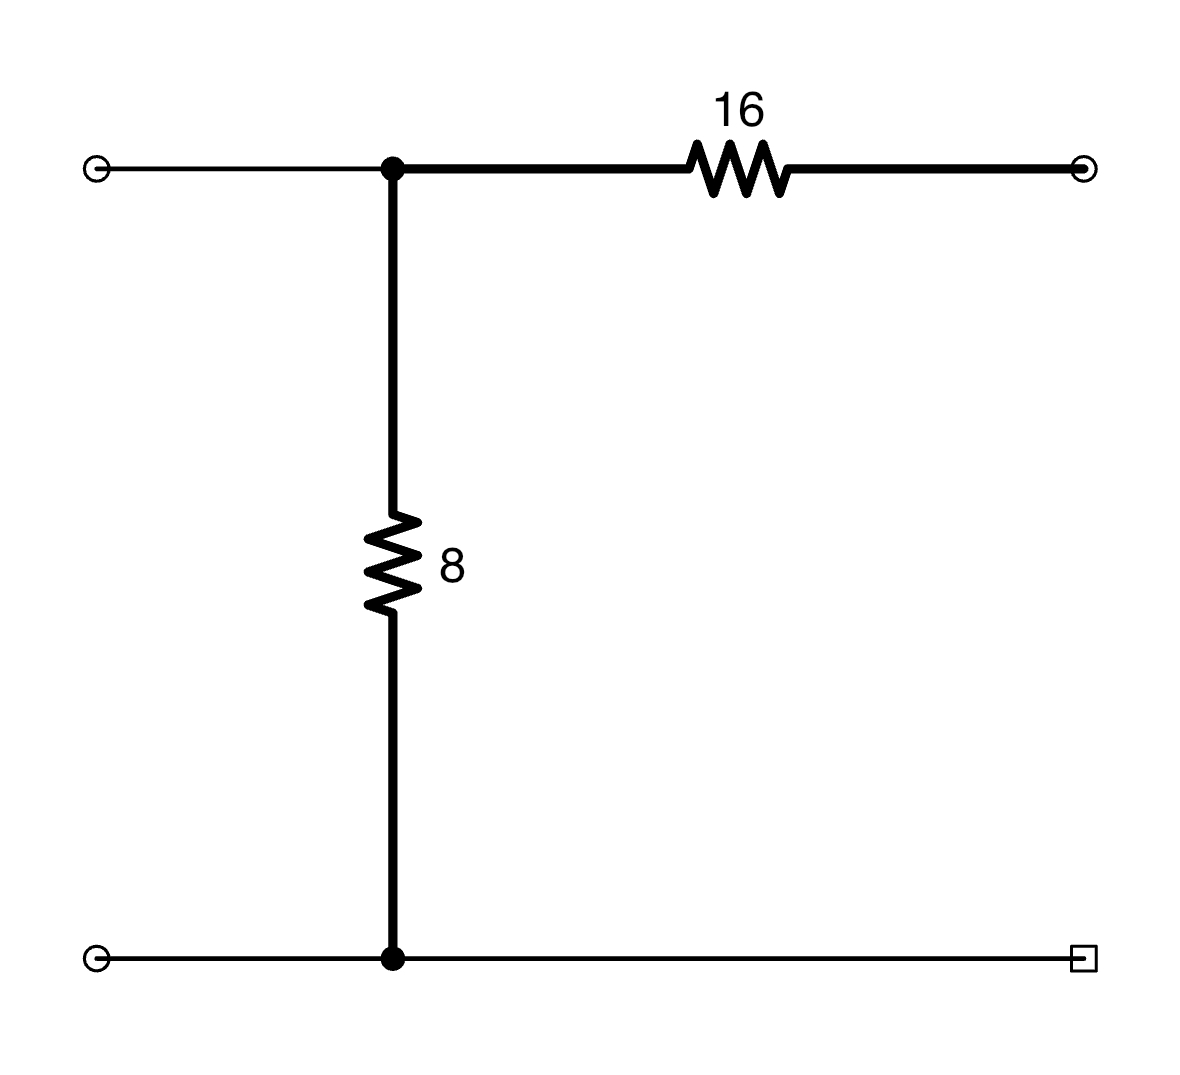
\includegraphics[width=60mm]{Image/19.jpg}
\end{figure}
\[R_N=16 \Omega +8 \Omega=24\]
\begin{figure}[H]
    \centering
    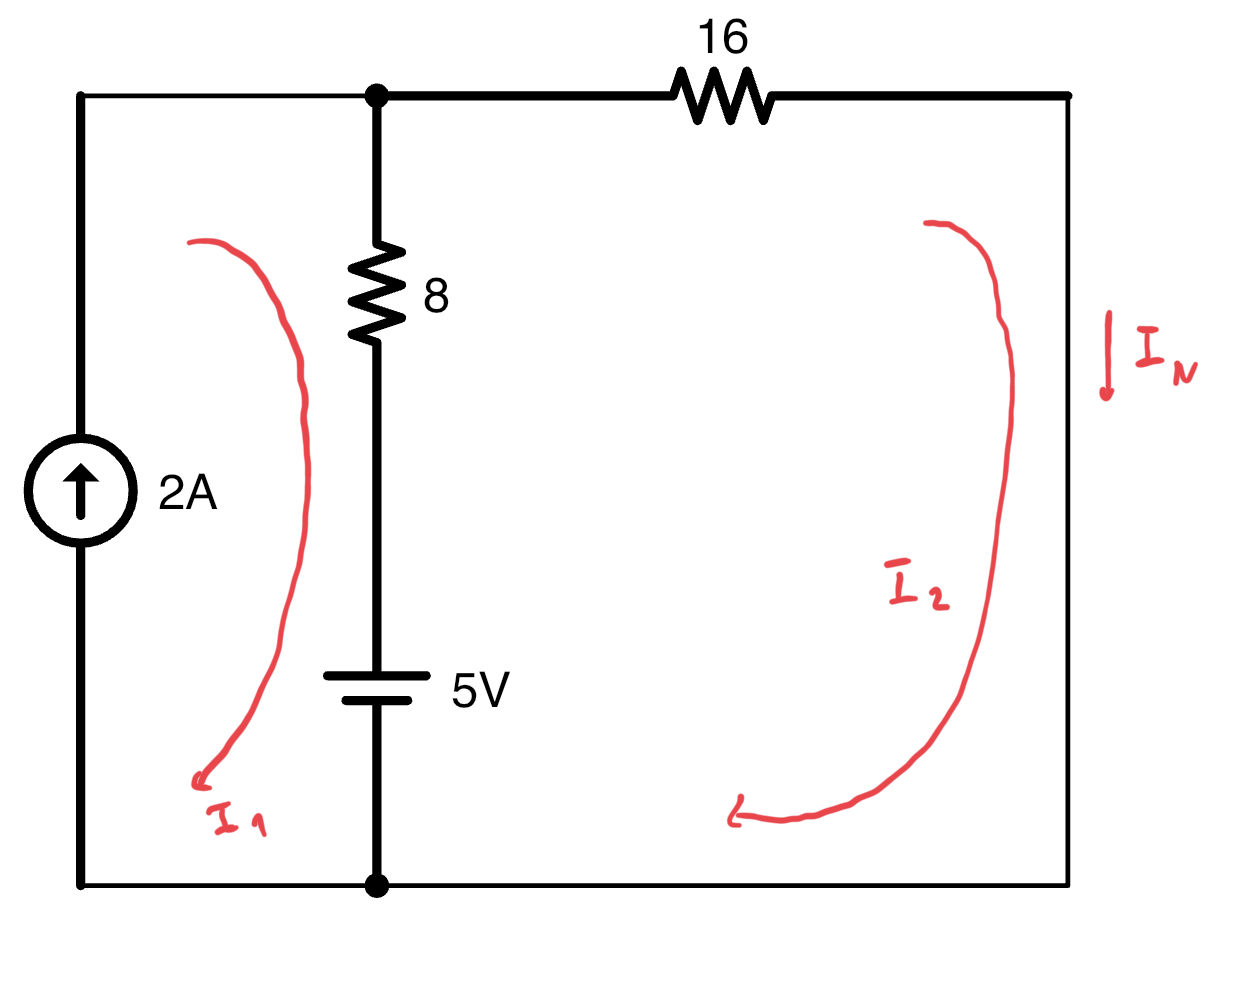
\includegraphics[width=100mm]{Image/20.jpg}
\end{figure}
\begin{gather}
    \sum V_{Loop 2}=8-8I_2+8I_1-16I_2=0\\
    8-8I_2+(8)(2)-16I_2=0\\
    24I_{2}=24\\
    I_2=1A\\
    I_L=(1A)(\frac{24\Omega}{24\Omega+R_L})\\
    \textbf{Second Method:}\\
    \sum I \rightarrow I_1+I_2+I_3=0\\
    2+\frac{8-V_1}{8}+0=0\\
    16+8-V_1=0\\
    V_1=24V\\
    I_N=\frac{24V}{24\Omega}=1A\\
    I_L=1A(\frac{24\Omega}{24\Omega +R_L})
\end{gather}
\subsection{Summery of Circuit Analysis:}

\begin{table}[H]
\centering
\begin{adjustbox}{}
\small
\begin{tabular}{|c|l|l|}
\hline
\textbf{Method}                                                                               & \multicolumn{1}{c|}{\textbf{Summery}}                                                           & \multicolumn{1}{c|}{\textbf{When to Apply}}                                                                     \\ \hline
\textbf{Mesh Analysis}                                                                        & \begin{tabular}[c]{@{}l@{}}KVL to obtain simultaneous \\ equation for the current\end{tabular}  & \begin{tabular}[c]{@{}l@{}}-Multiple currents are needed\\ -Current source are present\end{tabular}             \\ \hline
\textbf{Node Analysis}                                                                        & \begin{tabular}[c]{@{}l@{}}KCL to obtain simultaneous\\  equation for the voltages\end{tabular} & \begin{tabular}[c]{@{}l@{}}-Multiple voltage are needed\\ -Voltage source are present\end{tabular}              \\ \hline
\textbf{\begin{tabular}[c]{@{}c@{}}Thevenin and\\  Norton Equivalent \\ circuit\end{tabular}} & \begin{tabular}[c]{@{}l@{}}Simple equivalent circuits, \\ source transformation\end{tabular}    & \begin{tabular}[c]{@{}l@{}}Intermediate values not\\  important, only output \\ voltage or current\end{tabular} \\ \hline
\end{tabular}
\end{adjustbox}
\end{table}
\subsection{Source Transformation:}



\subsection{Maximum Power Transfer:}
We need to match the load resistor to system resistor for maximum power transfer.
\begin{gather}
    P=RI^2\\
    P=\frac{v_{TH}^2}{(R_{TH}+R_L)}R_L\\
    P=\frac{v_{TH}^2}{4R_{TH}}\rightarrow R_{TH}=R_L
\end{gather}
\subsection{Superposition:}
Total response a current on an element is a circuit is the sum of each independent source acting individually.\\
\textbf{Open the current source and short the voltage source.}
\begin{figure}[H]
    \centering
    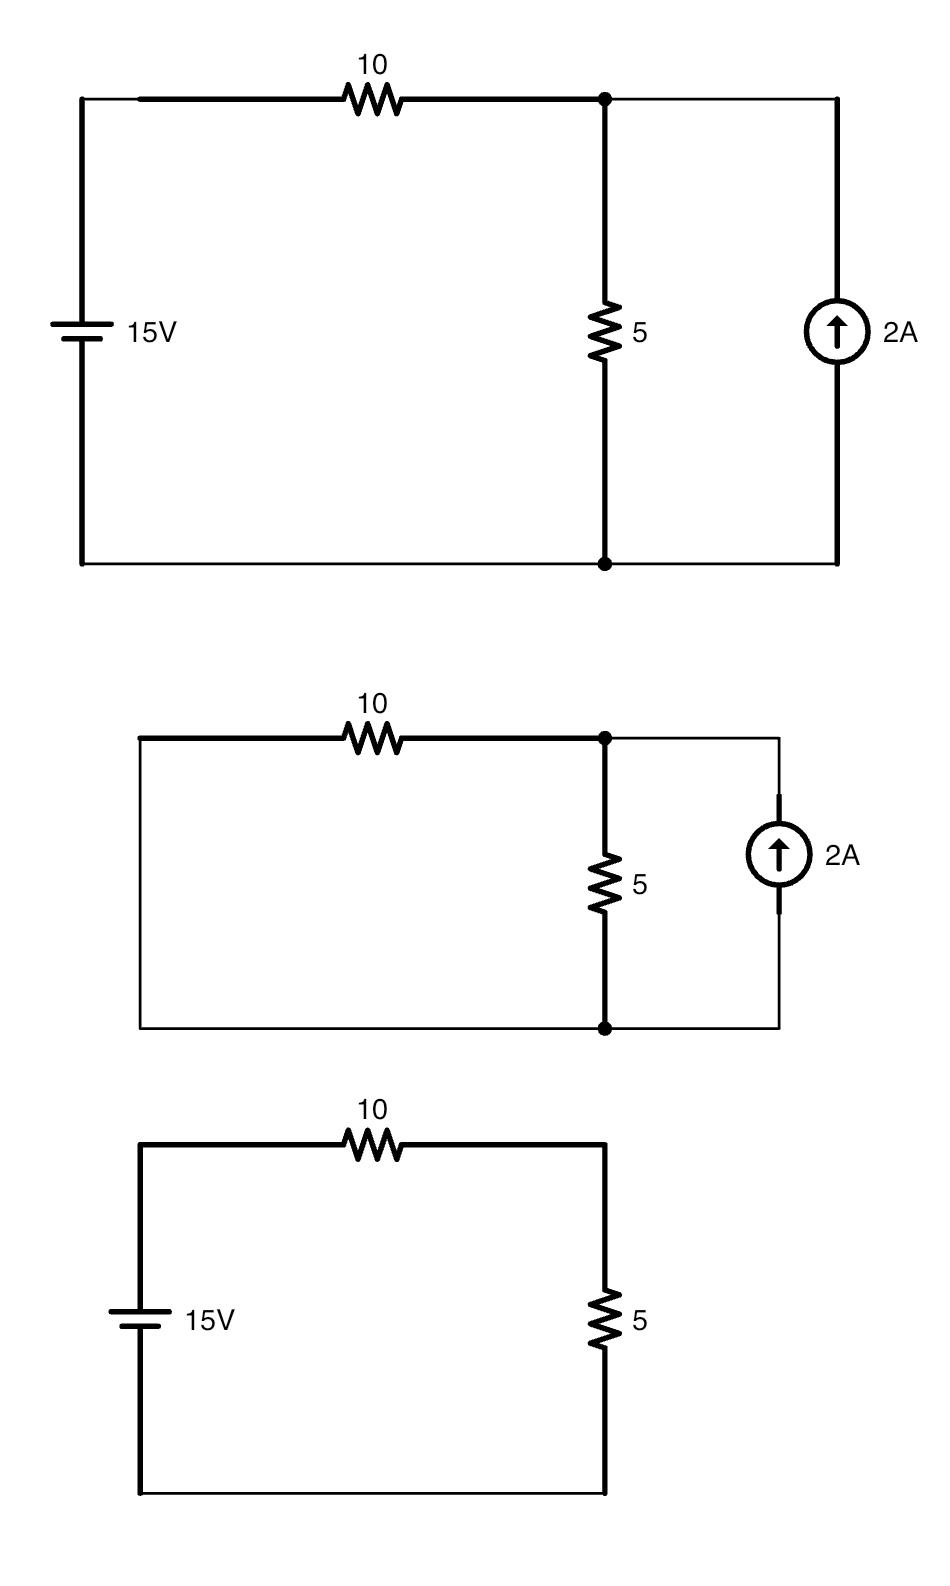
\includegraphics[width=50mm]{Image/21.jpg}
\end{figure}
\begin{gather}
    I_{R_1}=\frac{2A\times R_2}{R_2+R_1}=\frac{2A\times 5\Omega}{15\Omega}=\overleftarrow{0.667A}\\
    I_{R_2}=2A-0.667A=1.33A\downarrow\\
    \hline
    i=\frac{15v}{15\Omega}=1A\\
    I_{R_1}=\overrightarrow{1A}\\
    I_{R_2}=1A\downarrow\\
    I_{R_1}=1A-0.667A=\overrightarrow{0.33}A\\
    I_{R_2}=1.33A+1=2.33A\downarrow
\end{gather}

\section{Capacitor and Inductors:}
\subsection{First Order Differential Equation: }
\begin{gather}
    \frac{dy}{dt}+ay=K,y(0)\\
    y(t)=\frac{K}{a}(1-e^{-at})+y(0)e^{-at}, t>0
\end{gather}
\textbf{Note:} We can only use this formula if K and a our constant.\\

\textbf{Example:}\\
\setcounter{equation}{0}
\begin{gather}
    \frac{dy}{dt}+10y=20,y(0)=1\\
    y(t)=2(1-e^{-10t})+e^{-10t}\\
    \text{steady state}=2 \indent \& \indent \tau=\frac{1}{10}
\end{gather}

\subsection{RC $\&$  RL}
\begin{gather}
i_C(t)=C\frac{dV}{dt}\\
V_L(t)=L\frac{di}{dt}\\
C\frac{dv}{dt}+\frac{V}{R}=0\\
L\frac{di}{dt}+Ri=0\\
\end{gather}
  \textbf{Simple RC Circuit:}\\
        \begin{gather}
        i_C+i_R=0\\
        C\frac{dv}{dt}+\frac{V}{R}=0\\
        V(t)=V_0e^{\frac{-t}{RC}}\\
        \tau=RC
        \end{gather}
  
  \textbf{Example:}
  \begin{figure}[H]
  \centering
  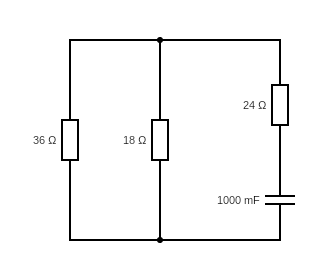
\includegraphics[width=80mm]{Image/29.jpeg}
  \end{figure}
  \begin{gather}
    Req=\frac{36*18}{36+18}+24=36\Omega \\
      \tau=RC=36\Omega \times 1F=36s\\
      V_C=10ve^{\frac{-t}{36}}\\
      V_B=\frac{12}{12+24}*10ve^{\frac{-t}{36}}=3.33e^{\frac{-t}{36}}
  \end{gather}
  \textbf{Example:}
  \begin{figure}[H]
      \centering
      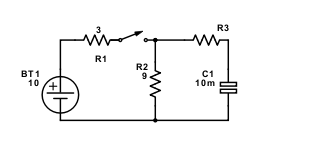
\includegraphics[width=120mm]{Image/30.png}
  \end{figure}
  \begin{gather}
      V_9=10*\frac{9\Omega}{3\Omega +9\Omega}=7.5V\\
       open\rightarrow V_c=7.5e^{\frac{-t}{0.1}}
  \end{gather}
  \textbf{Steps For Solving RC Circuit: }
  \begin{gather*}
      Steps\begin{cases}
      V_C(t=0) \indent V_C(t=\infty) \indent \tau=RC\\
      V_C(t)=V_C(\infty)+[V_C(0)-V_C(\infty)]e^{\frac{-t}{RC}}\\
      \end{cases}
  \end{gather*}
  \textbf{Example:}
  \begin{figure}[H]
      \centering
      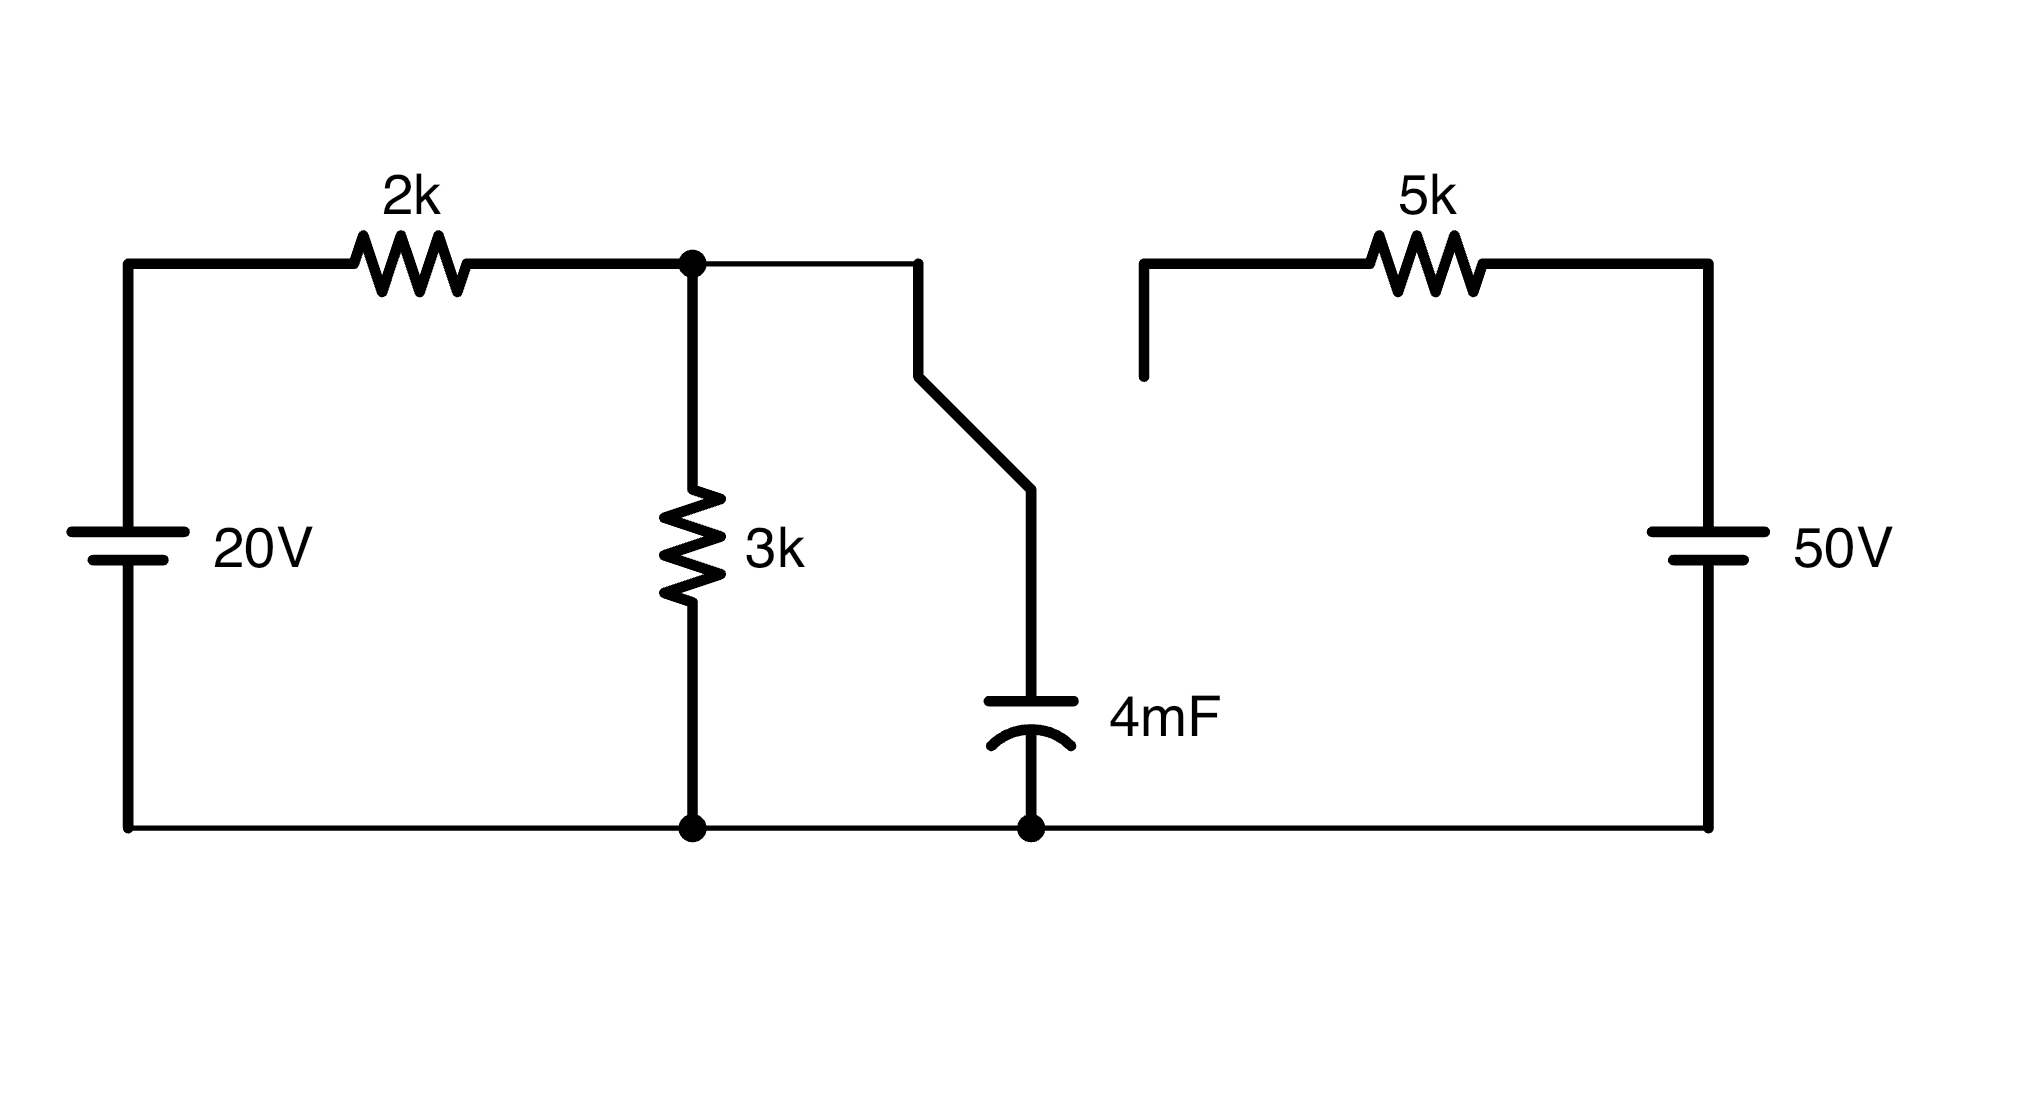
\includegraphics[width=120mm]{Image/33.jpeg}
  \end{figure}
  \begin{gather}
      V_C(t=0)=12v\\
      V_C(t=\infty)=50\\
      \tau=RC=5k\Omega *04mF=2sec\\
      V_C(t)=50v-[12-50]e^{\frac{-t}{2}}50-38e^{\frac{-t}{2}}
  \end{gather}
\subsection{Inductor:}
\[v=L \frac{di}{dt}\]
\[i(t)=\frac{V}{R}+(I_0-\frac{V}{R})e^{\frac{-t}{\tau}}\]
\textbf{Note:}\text{The inductor in \textbf{series} will $L_1+L_2$ to each other and in \textbf{parallel} $\frac{1}{L_1}+\frac{1}{L_2}=\frac{1}{L_T}$.}\\
\textbf{General Strategy:}
\begin{gather*}
    Steps=\begin{cases}
     i(t=0) \indent i(t=\infty) \indent \tau=\frac{L}{R}\\
     i(t)=i(t=\infty)+[i(t=0)-i(t=\infty)]e^{\frac{-t}{\tau}}
    \end{cases}
\end{gather*}
\textbf{Note:} if i(t=0)=0 we need use this formula: $i(t)=\frac{V}{R}(1-e^{\frac{-t}{\tau}})$\\
\textbf{Example:}
\begin{figure}[H]
    \centering
    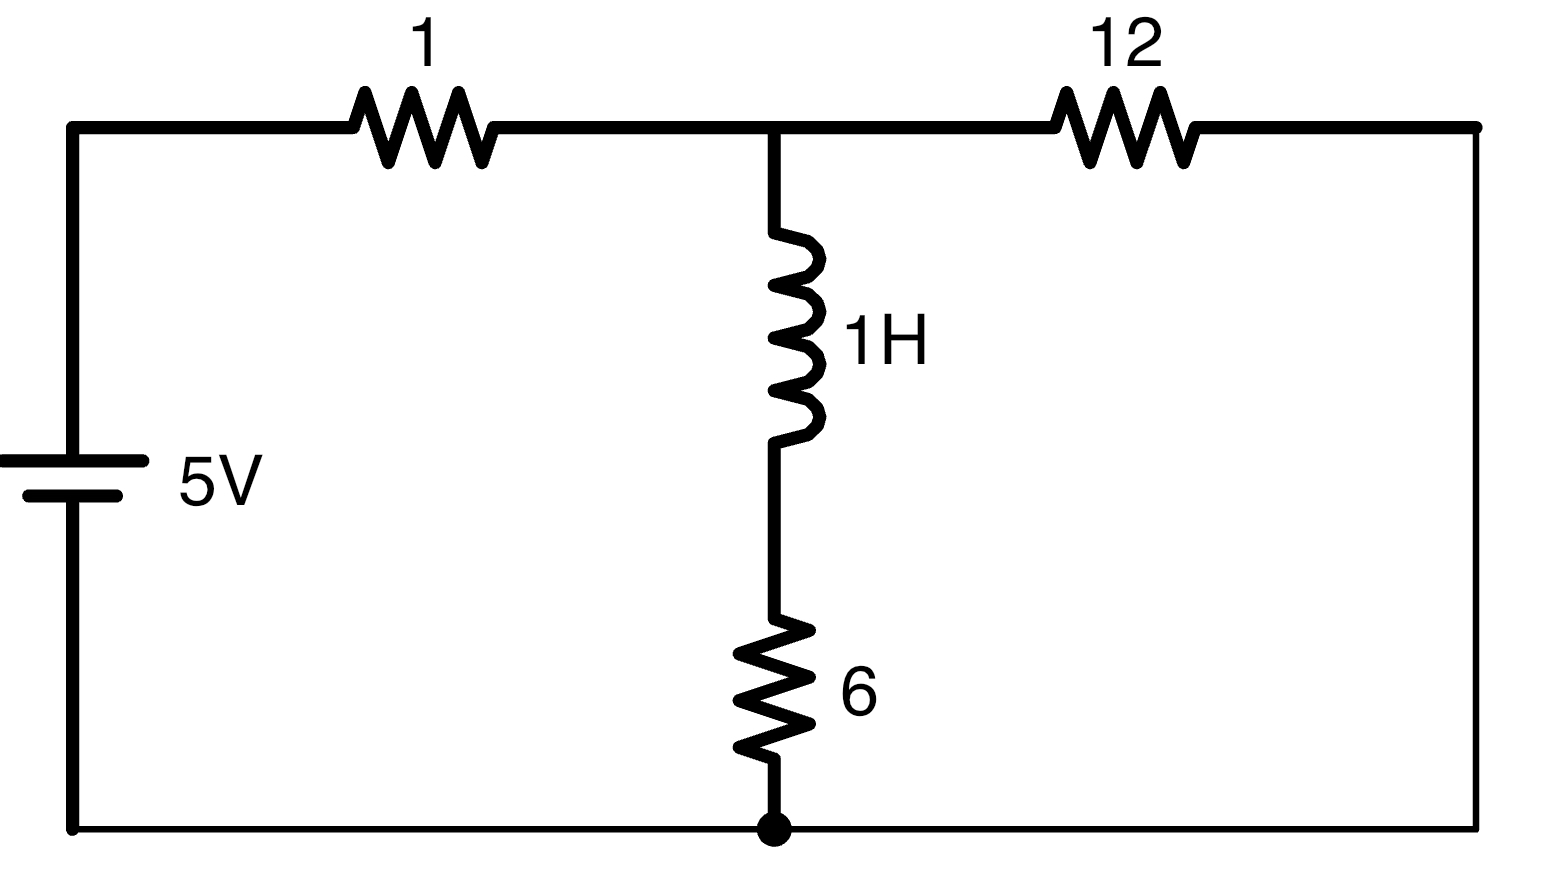
\includegraphics[width=100mm]{Image/22.jpeg}
\end{figure}
After while is act as a wire and current move to the inductor.\\
\begin{gather}
    P(t)=v(t)v(t)\\
    w(t)=\int _{t_0}^{t}p(\tau)d\tau +w(t_0)\\
    v=L \frac{di}{dt}\\
    w=\frac{1}{2}Li^2
    \end{gather}
   % \newpage
    \textbf{Example:}\\
    \begin{figure}[H]
        \centering
        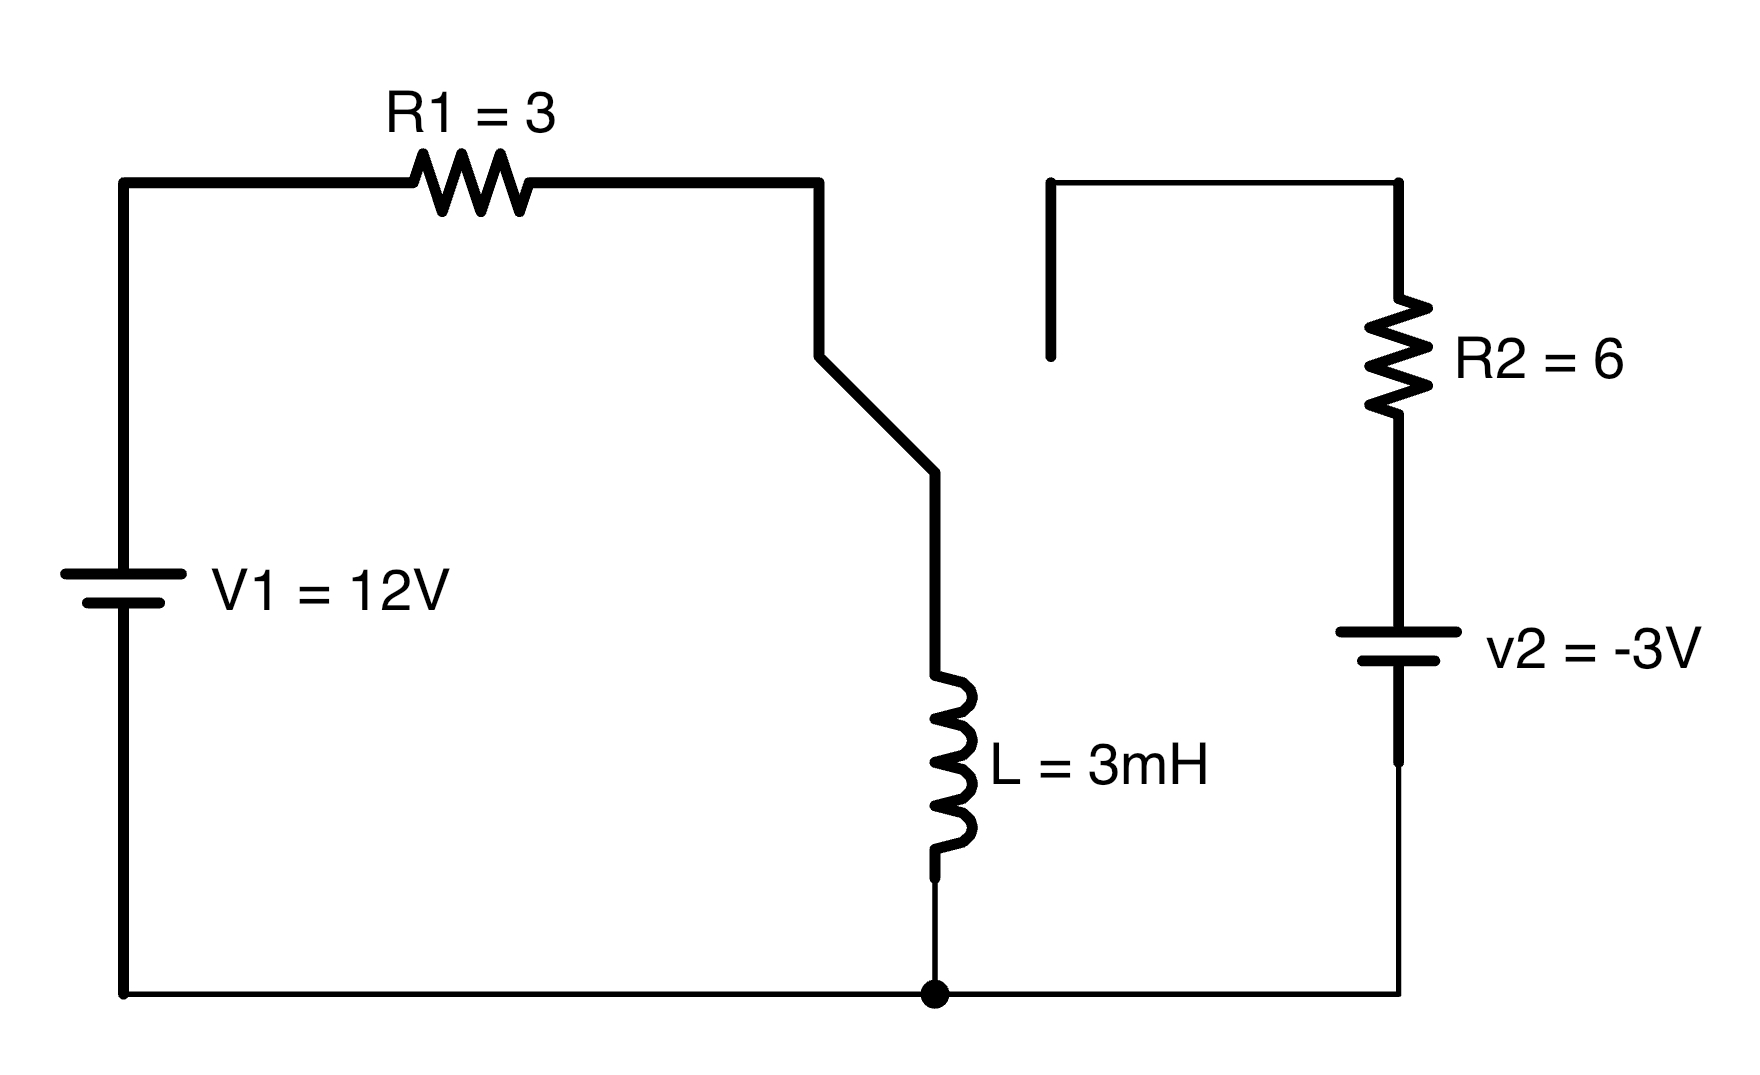
\includegraphics[width=120mm]{Image/23.jpeg}
    \end{figure}
    \begin{gather}
        i_L=\frac{v_2-v_L}{R_2}\\
        i_L=\frac{v_2-L\frac{di_L}{dt}}{R_2}\\
        \frac{di_L}{dt}+\frac{t_2}{L}i_L=\frac{v_2}{L}\\
        \tau=\frac{L}{R_2}\\
         i_L=\frac{v_2}{R_2}[1-e^{\frac{-t}{\tau}}]+\frac{v_1}{R_1}e^{\frac{-t}{\tau}}
        \end{gather}
      
        \textbf{Example:}
    \begin{figure}[H]
        \centering
        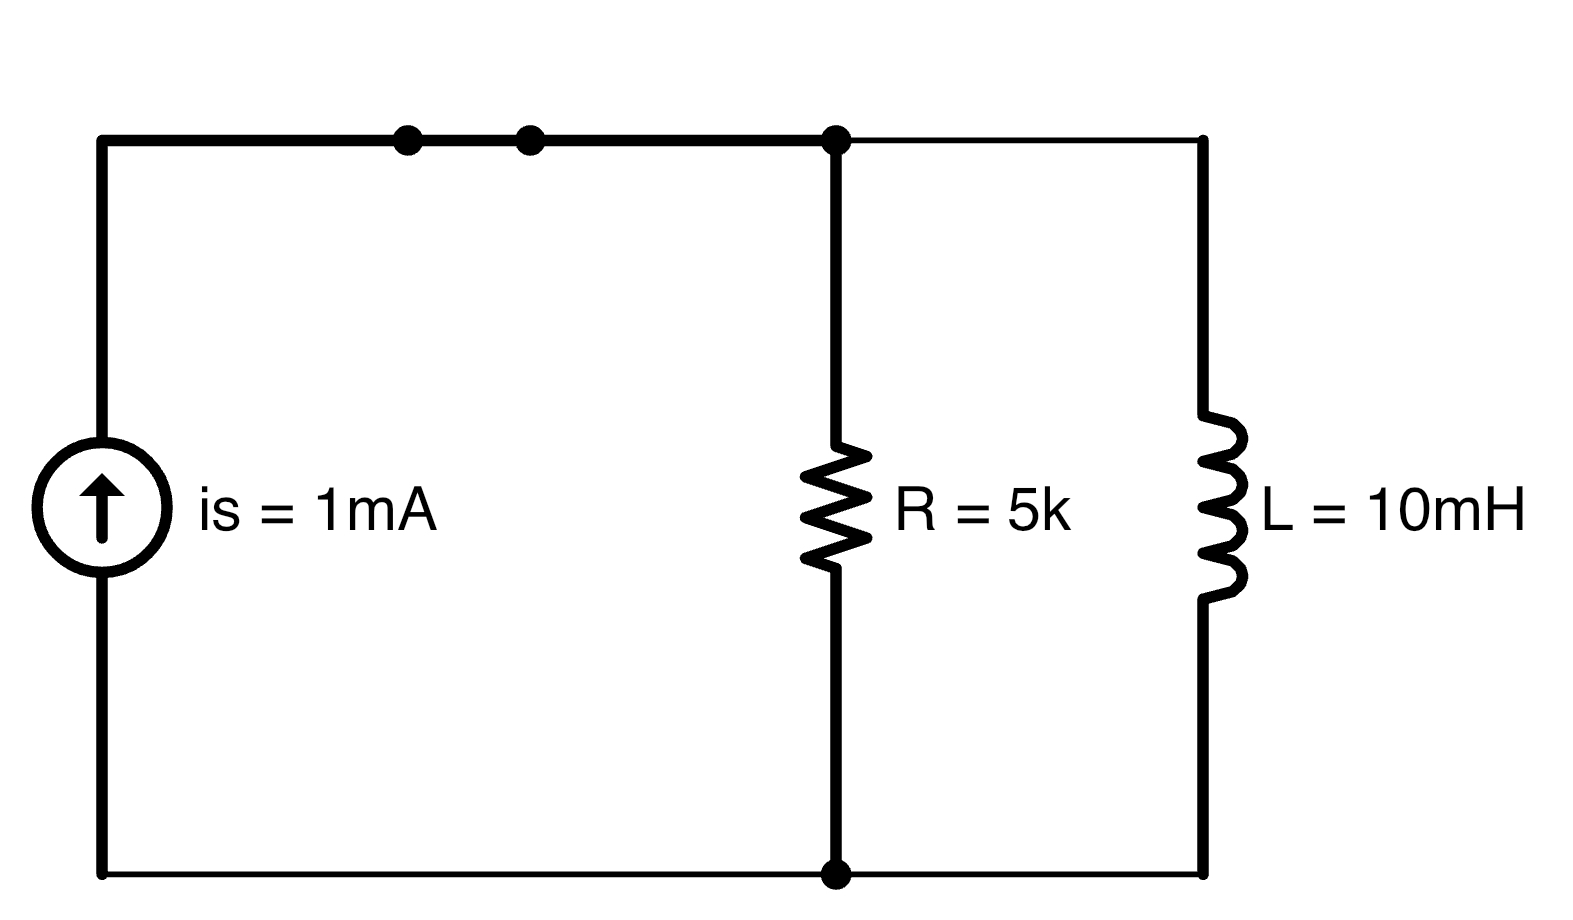
\includegraphics[width=83mm]{Image/24.jpeg}
    \end{figure}
    \begin{gather}
      i_R=\frac{v_L}{R}\\
      i_s=i_r+i_L\\
      i_s=\frac{L}{R}\frac{di_L}{dt}+i_L\\
      \frac{di_L}{dt}+\frac{R}{L}i_L=\frac{R}{L}i_s\\
      \tau=\frac{L}{R}\\
      i_L=i_s[1-e^{\frac{-t}{\tau}}]\\
      v_L=i_sRe^{\frac{-t}{\tau}}
    \end{gather}
    \textbf{Example:}
    \begin{figure}[H]
    \centering
    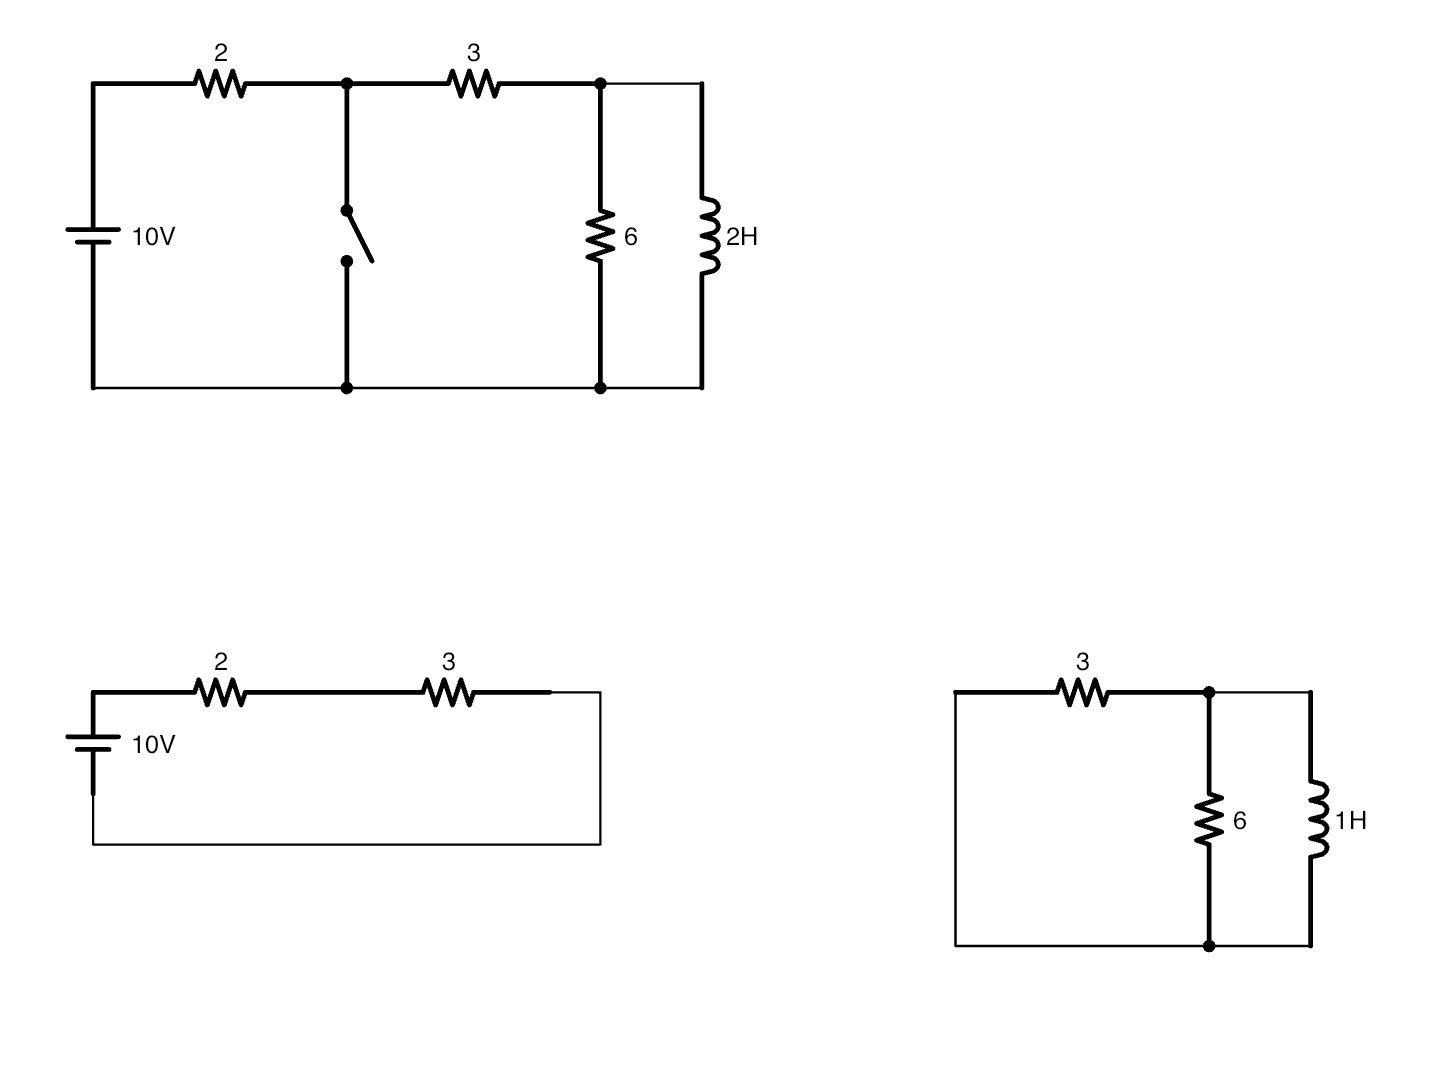
\includegraphics[width=150mm]{Image/31.jpeg}
\end{figure}
\begin{gather}
    I_L=\frac{V}{R}=\frac{10V}{5\Omega}=2A\\
    \tau=\frac{L}{R}=\frac{2H}{2\Omega}=1sec\\
    I_L(t)=2Ae^{-t}\\
    V_L=L\frac{di}{dt}\\
    V_L=2H\frac{d}{dt}[2Ae^{-t}]=-4Ve^{-t}\\
    I_6=\frac{V_6}{R}=\frac{-4Ve^{-t}}{6\Omega}=\frac{-2}{3}*e^{-t}
\end{gather}
\textbf{Example:}
\begin{figure}[H]
    \centering
    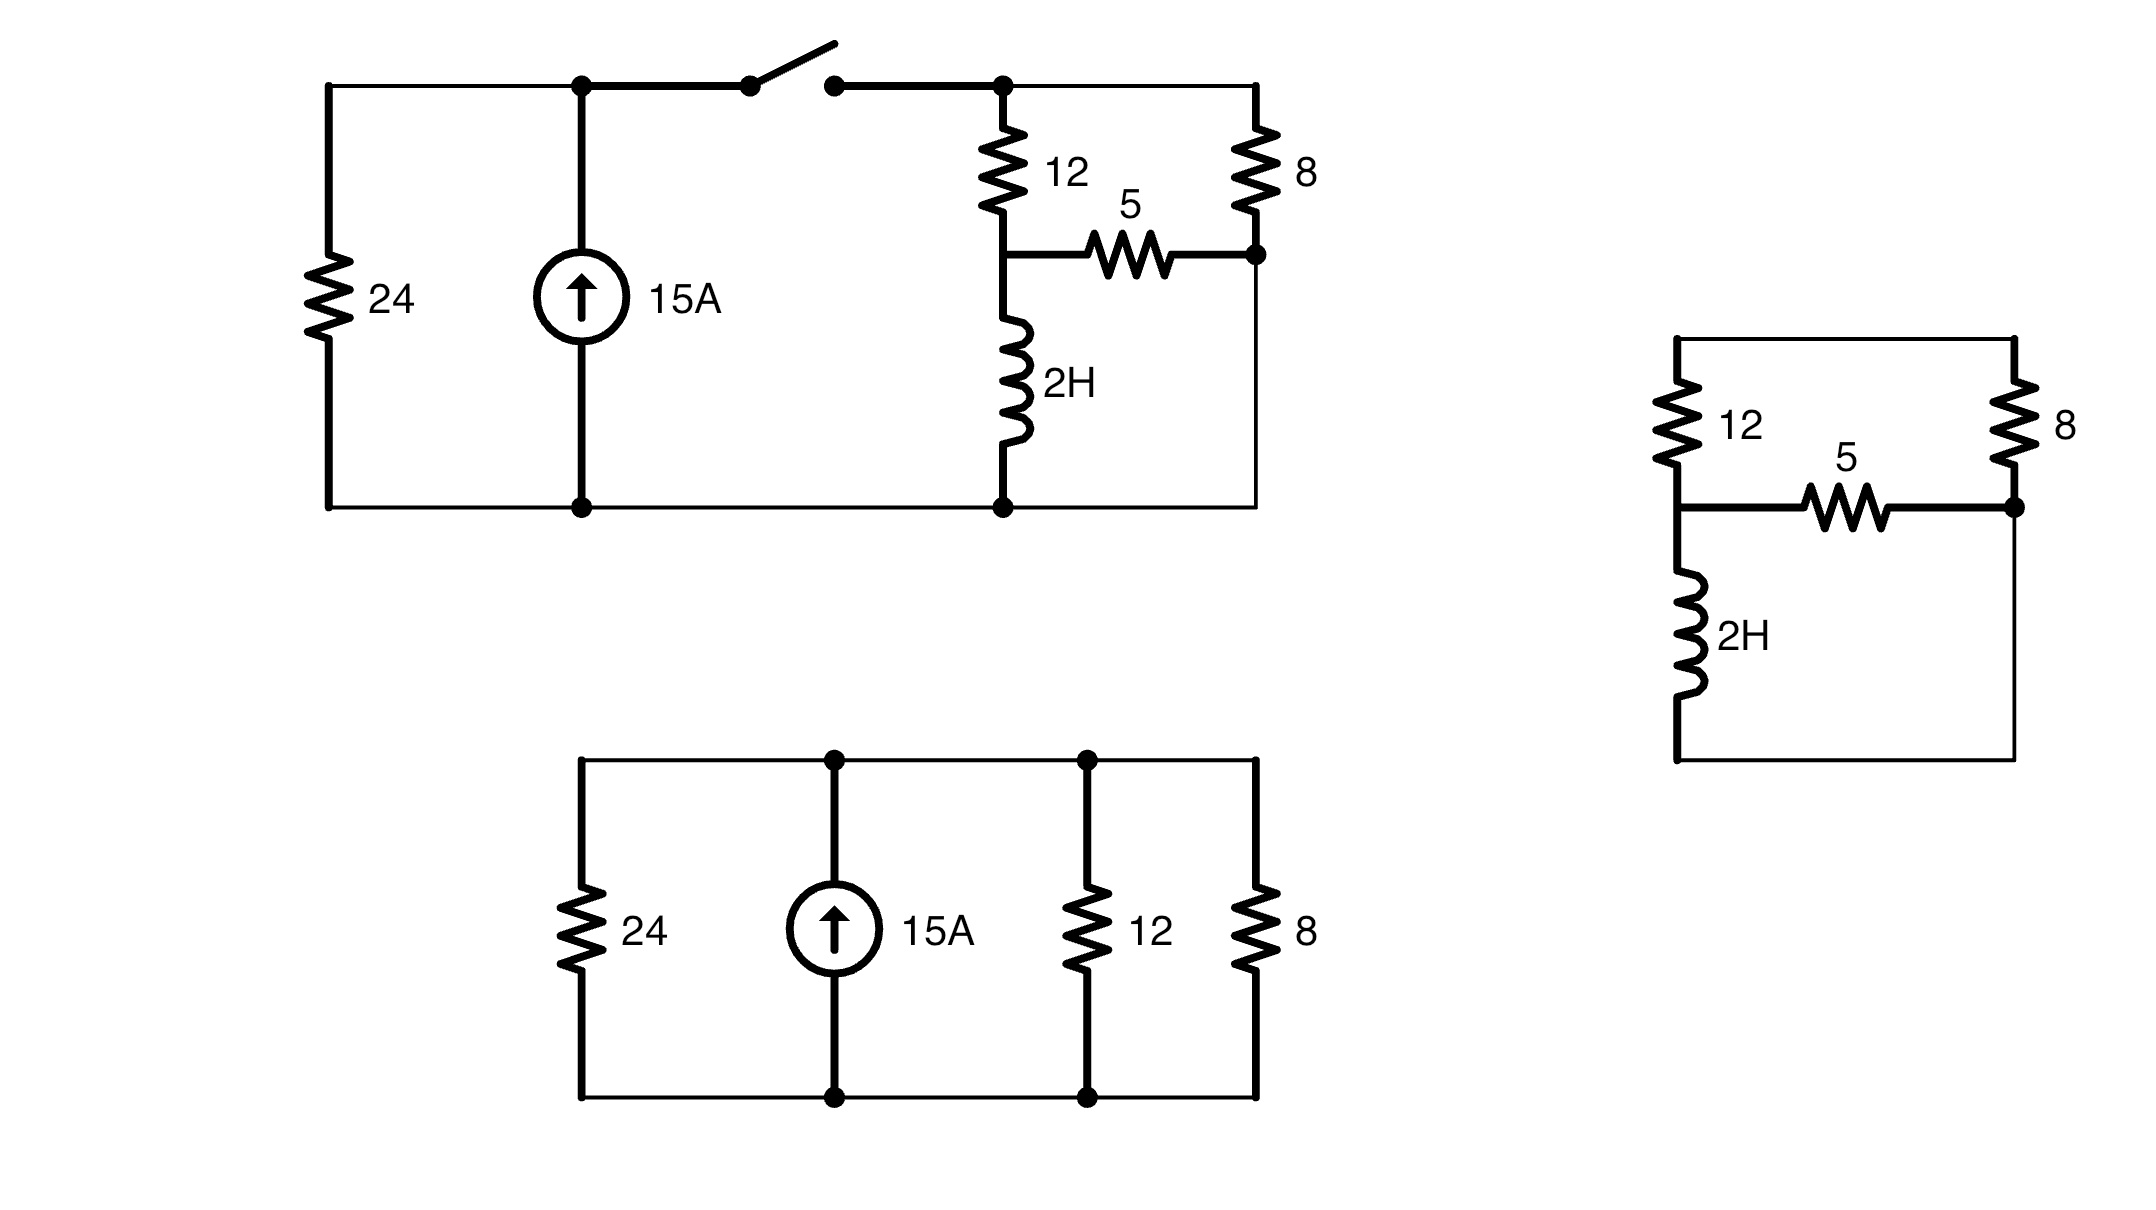
\includegraphics[width=150mm]{Image/32.jpeg}
\end{figure}
\begin{gather}
    I_1=15*\frac{12*8}{12*8+12*24+8*24}=2.5A\\
    I_2=15*\frac{24*8}{12*8+12*24+8*24}=5A\\
    I_3=15*\frac{12*24}{12*8+12*24+8*24}=7.5A\\
    \tau=\frac{2H}{4\Omega}=0.5sec\\
    I_L(t)=5Ae^{-2t}\\
    V_L(t)=2*(-10ve^{-2t})=-20ve^{-2t}
\end{gather}
\textbf{Example:}
\begin{figure}[H]
    \centering
    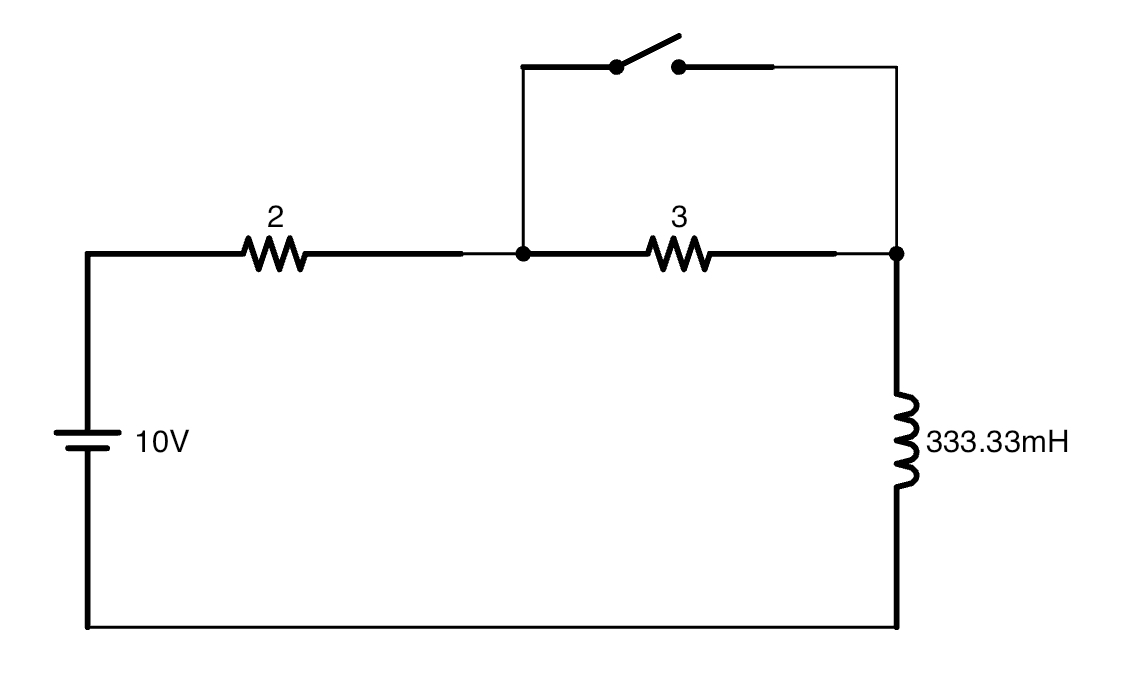
\includegraphics[width=120mm]{Image/34.jpeg}
\end{figure}
\begin{gather}
    i(t=0)=\frac{10}{2}=5\\
    i(t=\infty)=\frac{10}{5}=2\\
    \tau=\frac{1}{15}sec\\
    i(t)=i(t=\infty)+[i(t=0)-i(t=\infty)]e^{\frac{-t}{\tau}}\\
    i(t)=2+(5-2)e^{-15t}\\
    i(t)=2A+3e^{-15t}\\
    10V-(2\Omega +3\Omega)i-L\frac{di}{dt}\\
    10v-5\Omega (2A+3e^{-15t})-\frac{1}{3}(-45Ae^{-15t})\\
    0=0
\end{gather}
    \newpage
 \subsection{Formula Sheet for Capacitance and Inductor:}
 
 \begin{multicols}{2}
 \underline{Capacitance:}
 \begin{gather}
    q=cv\\
    i(t)=c\frac{dv}{dt}\\
    v(t)=\frac{1}{c}\int _0^t i(t)dt+v_0\\
    P=cv\frac{dv}{dt}\\
    w(t)=\frac{1}{2}cv^2(t)\\
    discharging\rightarrow v(t)=v_i e^{-\frac{t}{\tau}}\\
    charging\rightarrow v(t)=v_s(1- e^{\frac{-t}{\tau}})\\
    \tau=RC 
 \end{gather}
 
\columnbreak

\underline{Inductor:}
\begin{gather}
v(t)=L\frac{di}{dt}\\
i(t)=\frac{1}{L}\int_0^t v(t)dt+i_0\\
P=Li\frac{di}{dt}\\
W=\frac{1}{2}Li^2(t)\\
    Discharging\rightarrow i(t)=\frac{v_s}{R_1}e^{\frac{-t}{\tau}}\\
    Discharging\rightarrow v(t)=L\frac{v_s}{R_1\tau}e^{\frac{-t}{\tau}}\\
   Discharging\rightarrow  \tau=\frac{L}{R_2}\\
   charging\rightarrow i(t)=\frac{v_s}{R_1}(1-e^{\frac{-t}{\tau}})\\
   charging\rightarrow v(t)=v_s e^{\frac{-t}{\tau}}
\end{gather}
 \end{multicols}\hrule
\subsection{RLC Circuit:}
\textbf{Example:}
\begin{figure}[H]
    \centering
    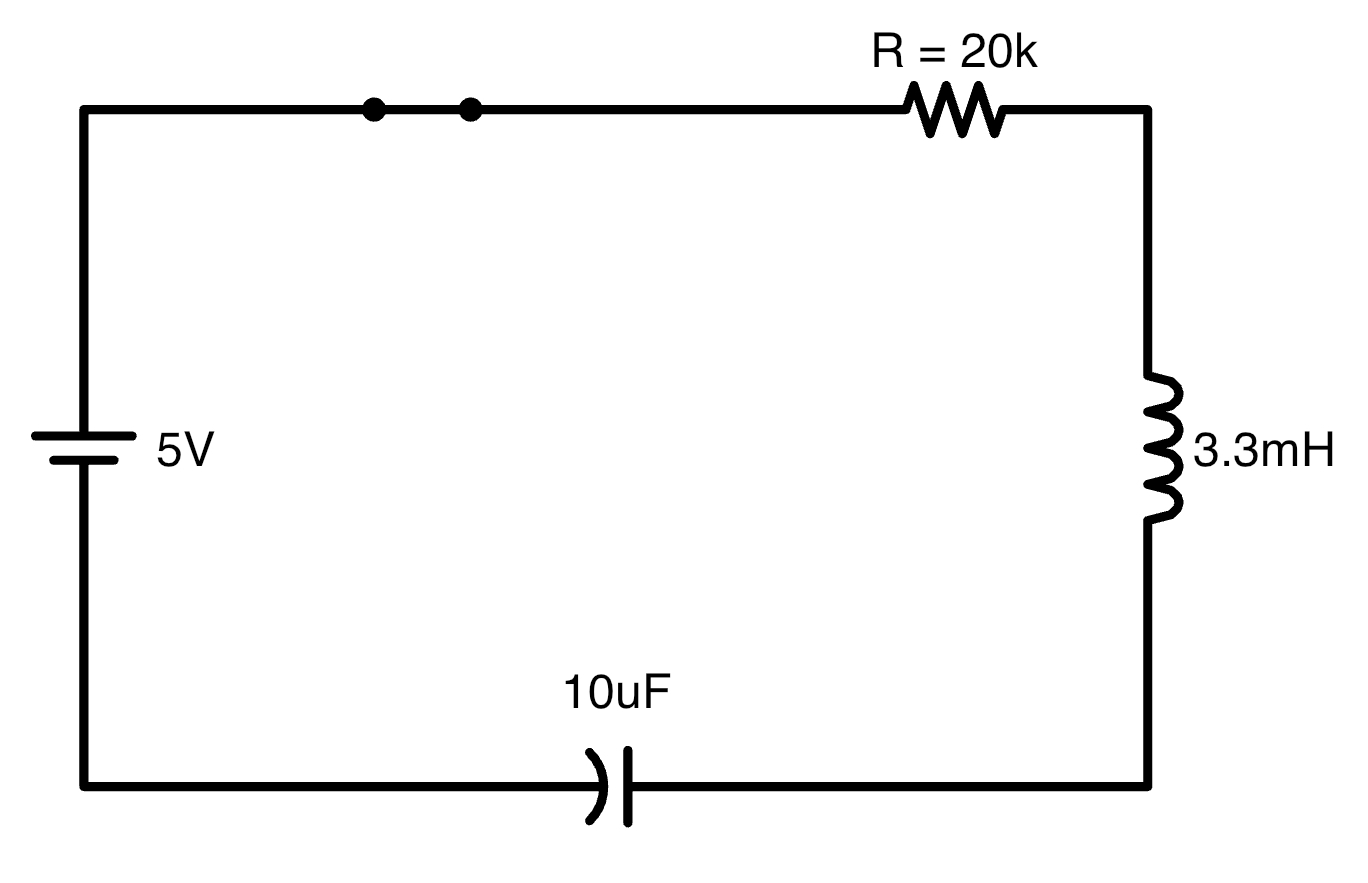
\includegraphics[width=80mm]{Image/25.jpeg}
\end{figure}
\textbf{Transient Response:}
\begin{gather}
    i(0^-)=0\\
    v_c(0^+)=0\\
    v_s=v_R+v_L+v_c\\
    v_R=iR\\
    v_L=L\frac{di}{dt}\\
    i=C\frac{dv_c}{dt}\\
    v_S=LC\frac{d^2v_c}{dt^2}+RC\frac{dv_c}{dt}+v_c\\
    \frac{d^2v_c}{dt^2}+\frac{R}{L}\frac{dv_c}{dt}+\frac{1}{L}v_c=\frac{v_s}{LC}\\
    \frac{d^2v_c}{dt^2}+6.06e-6{L}\frac{dv_c}{dt}+30.3e9v_c=151.5e9\\
    v_{c,t}=K_1e^{-5.00e3t}+K_2e^{-6.06e6t}
\end{gather}
\textbf{Steady State:}
\begin{gather}
    v_c\rightarrow \frac{k}{a_2}=LC\frac{v_s}{LC}=v_s\\
    v_{c,s}=5
\end{gather}
\textbf{Sum of the $V_c$:}
\begin{gather}
v_c=v_{c,t}+v_{c,s}\\
v_c=K_1e^{-5.00e3t}+K_2e^{-6.06e6t}+5\\
v_c(0^-)=v_c(0)=0\\
K_1+K_2+5=0\\
i(0^-)=0\\
i=C\frac{dv_c}{dt}\\
-50e-6K_1-60.6e-3K_2=\\
K_1=-5.00413 \indent \& \indent K_2=0.00413
\end{gather}
\subsection{Second Order circuit:}
\begin{gather}
	\frac{d^2x}{dt^2}+2\alpha \frac{dx}{dt}+\omega^2=f(t)\\
	s^2+2\alpha s+\omega_0=0\\
	\zeta =\frac{\alpha}{\omega}\\
	s_1=-\alpha+\sqrt{\alpha^2-\omega_0 ^2}\\
	s_2=-\alpha-\sqrt{\alpha^2-\omega_0 ^2}\\
	x_c=K_1e^{s_1t}+K_2e^{s_2t}\rightarrow \zeta>1\text{ overdamped}\\
	x_c=K_1e^{s_1t}+K_2te^{s_1t}\rightarrow \zeta=1\text{ critically damped}\\
	x_c=K_1e^{-\alpha t}cos(\omega_n t)+K_2e^{-\alpha t}sin(\omega _n t)\rightarrow \zeta<1 \text{ underdapmped}\\
	\omega _n=\sqrt{\omega _0^2-\alpha^2}\\
	\alpha=\frac{1}{2RC}\\
	\omega _0=\frac{1}{\sqrt{LC}}
\end{gather}
\subsection{Steps for Solving RLC:}
\begin{equation}
    \begin{cases}
    i(t=0^-) \indent V(t=0^-)\\
    i(t=0^+) \indent V(t=0^+)\\
     \frac{di}{dt}(t=0^+) \indent \frac{dv}{dt}(t=0^+)\\
     i_L(t\rightarrow \infty) \indent V_C(t \rightarrow \infty)
    \end{cases}
\end{equation}
\clearpage
\section{Steady State Sinusoidal Analysis:}
\subsection{sinusoidal currents and voltage:}

    \[v(t)=V_m cos(\omega t_\theta)\]
    $V_m$ is the \textbf{peak value} and $\omega$ is the \textbf{angular frequency} in radians per second and $\theta$ is the \textbf{phase angle}.\\
    \begin{gather}
       \omega = \frac{2\pi}{T}\\
    f=\frac{1}{T}\rightarrow \omega =2\pi f\\
    V_{rms}=\sqrt{\frac{1}{T}\int_0^T V_m^2\cos^2(\omega t+\theta)dt} \\
    V_{rms}=0.707 V_m\rightarrow sinusoidal
    \end{gather}
   \subsection{Phasor Representation of Sinusoidal:}
   \begin{gather}
       V(c)=v_m cos(\omega t+\theta)\\
       \text{Phasor}\rightarrow v_m\angle\theta\\
       Regtangular\rightarrow V_m \cos{\theta}+j V_m \sin{\theta}
   \end{gather}
   \textbf{Note:} sin wave represented by phasor allows easy multiplication and division. \\
   \textbf{Note:} sin wave represented by rectangular allows easy addition and subtraction.\\
   \textbf{Example:} our supply PGE 60HZ and 120 $V_{rms}$. Write instantaneous, polar, and rectangular?\\
   \begin{enumerate}
       \item convert frequency to radian.
       \item calc $V_p$ or $V_max$.
       \item write instantenous 
       \item write polar
       \item write rectangular
   \end{enumerate}
   \begin{gather}
        \omega=2\pi*60HZ=377\\
       V_p=\frac{V_{rms}}{0.707}=\frac{120}{0.707}=170V\\
       polar:170\angle 0^\circ\\
       rect:170\cos{0}+j170\sin{0}\\
       inst:v=170cos(377t+0)
   \end{gather}
   \textbf{Example:} give assume rect,polar,instantaneous.
   \begin{gather}
       V_1=200cos(\omega t+60)\\
       V_{1polar}=200\angle60\\
       V_2=100sin(\omega t-20)\\
       V_2=100cos(\omega t-20-90)=100cos(\omega t-110)\\
       V_{2Polar}=100\angle-110\\
       V_1=200cos(60)+j200sin(60)\\
       V_2=100cos(-110)+j100sin(-110)\\
       V_1+V_2=(100-34)+(173-94)j\\
       \boxed{V_1+V_2=66+79j}\\
       V_T=\sqrt{66^2+79^2}=102.94\\
       \boxed{V_{add}=102.94cos(\omega t+50.12)}\\
       \boxed{polar:102.94\angle 50.12}\\
       V_1-V_2=(100+34)+(173+94)j\\
       \boxed{V_{sub}=134+267j}\\
       V_{maxSub}=\sqrt{134^2+267^2}=298.73\\
       \boxed{V=298.73cos(\omega t+63.35)}\\
       \boxed{polar:298.73\angle 63.35}\\
       \boxed{Division:\frac{200\angle60}{100\angle-110}=2\angle{60-(-110)}=2\angle170}\\
       \boxed{V=2cos(\omega t+170)}\\
       \boxed{2cos(170)+j2sin(170)=-1.96+0.348j}\\
       \boxed{Multiplication:200\angle60*100\angle-110=20000\angle-50}\\
       \boxed{V_{multiplication}=20000cos(\omega t-50)}\\
       \boxed{20000cos(-50)+20000sin(-50)j=12855-15321j}
   \end{gather}
   \subsection{Complex Impedances:}
    \begin{gather}
        i_L(t)=I_m sin(\omega t+\theta)\rightarrow I_L=I_m\angle \theta -90^\circ\\
        V_L(t)=\omega L I_m cos(\omega t+ \theta)\rightarrow V_L=\omega L I_m\angle \theta=V_m\angle \theta\\
        Z_L=j \omega L=\omega L\angle 90\\
        V_L=Z_LI_L
    \end{gather}
    \subsection{Capacitance:}
    \begin{gather}
        V_C=Z_CI_C\\
        Z_C=-j \frac{1}{\omega C}=\frac{1}{j\omega C}=\frac{1}{\omega C}\angle-90^\circ\\
    \end{gather}
    \subsection{Circuit Analysis Using Phasors and Impedances:}
    \begin{enumerate}
        \item Replace the time descriptions of the voltage and current sources with the corresponding phasors.(All of the sources must have the same frequency.)
        \item Replace inductances by their complex their complex impedances $Z_L$. Replace campcitances by their complex impedances $Z_C$.Resistance have impedances equal to their resistance.
        \item Analyze the circuit by using any of the techniques which we studied.
    \end{enumerate}
    \textbf{Example: }Find the steady-state current for the circuit shown. Also, find the phasor voltage across each element and construct a phasor diagram.
    \begin{figure}[H]
        \centering
        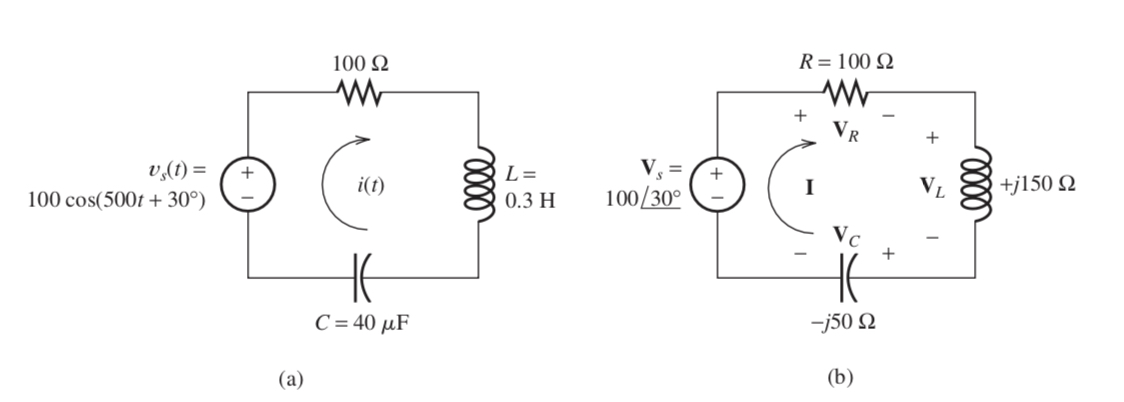
\includegraphics[width=140mm]{Image/26.jpeg}
    \end{figure}
    \begin{gather}
        V_s=100\angle 30^\circ\\
        Z_L=j\omega L=j500\times 0.3=j150\Omega\\
        Z_c=-j\frac{1}{500\times 40\times 10^{-6}}=-50j\Omega\\
        Z_{eq}=R+Z_L+Z_C=100+j150-j50=100+j100\\
        Z_{eq}=141.4\angle 45^\circ\\
        I=\frac{V_s}{Z}=\frac{100\angle 30^\circ}{141.4\angle 45^\circ}=0.707\angle-15^\circ\\
        i(t)=0.707cos(500t-15^\circ)\\
       \star V_R=R\times I=100\times 0.707\angle-15^\circ=70.7\angle-15^\circ\\
       \star V_L=\omega L\angle90^\circ I=150\angle 90^\circ\times 0.707\angle-15^\circ=106.1\angle75^\circ\\
       \star V_C=\frac{1}{\omega C}\angle-90^\circ I=50\angle-90^\circ\times0.707\angle-15^\circ=35.4\angle-105^\circ
    \end{gather}
    \begin{figure}[H]
        \centering
        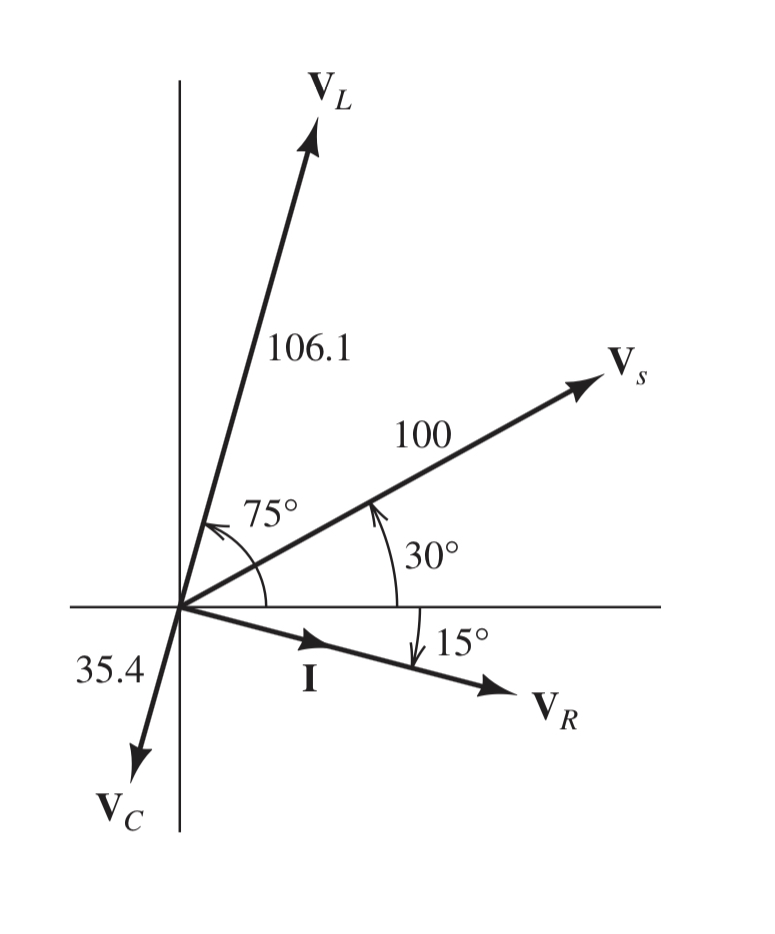
\includegraphics[width=70mm]{Image/27.jpeg}
    \end{figure}
    \cleardoublepage
     \textbf{Example: }Find the voltage $V_C(t)$ in the steady state. Also, find the phasor voltage across each element and construct a phasor diagram.
     \begin{figure}[H]
         \centering
         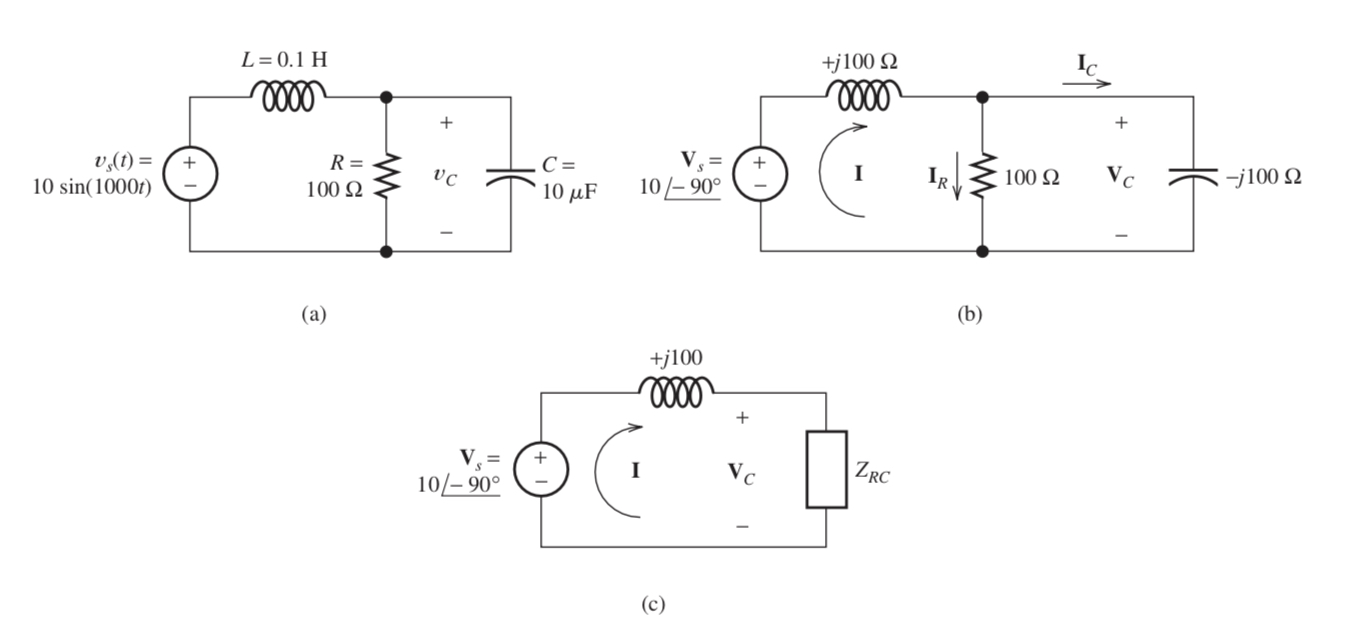
\includegraphics[width=170mm]{Image/28.jpeg}
     \end{figure}
     \begin{gather}
         V_s=10\angle-90^\circ\\
         Z_L=j\omega L=j1000\times 0.1=j100\Omega\\
         Z_C=-j\frac{1}{1000\times 10\times 10^{-6}}=-j100\Omega\\
         Z_{RC}=\frac{1}{\frac{1}{R}+\frac{1}{Z_C}}=\frac{1}{\frac{1}{100}+\frac{1}{-j100}}=\frac{1}{0.1+j0.01}=\frac{1\angle 0^\circ}{0.01414\angle45^\circ}=70.71\angle -45^\circ\\
         V_C=V_S\frac{Z_{RC}}{Z_L+Z_{RC}}=10\angle-90\frac{70.71\angle-45}{j100+50-50j}=10\angle-180^\circ\\
         V_C(t)=10cos(1000t-180^\circ)=-10cos(1000t)\\
         I=\frac{V_S}{Z_L+Z_{RC}}=\frac{10\angle-90}{j100+50-j50}=0.1414\angle-135^\circ
     \end{gather}
     \section{Fourier Series:}
     \begin{gather}
         f(t)=a_0+\sum _{n=1}^\infty(a_n cos(n\omega t)+b_nsin(n\omega t)\\
         a_0=\frac{1}{T}\int_1^T f(t)dt\\
         a_n=\frac{2}{T}\int_0^T f(t)cos(n\omega t)dt\\
          b_n=\frac{2}{T}\int_0^T f(t)sin(n\omega t)dt\\
           f(t)=a_0+\sum _{n=1}^\infty A_n cos(n\omega t+\phi _n)\\
           A_n=\sqrt{a_n^2+b_n^2}\\
           \phi _n=-tan^{-1}(\frac{b_n}{a_n})\\
           A_n\angle \phi_n=a_n-jb_n
     \end{gather}
     \begin{figure}[H]
         \centering
         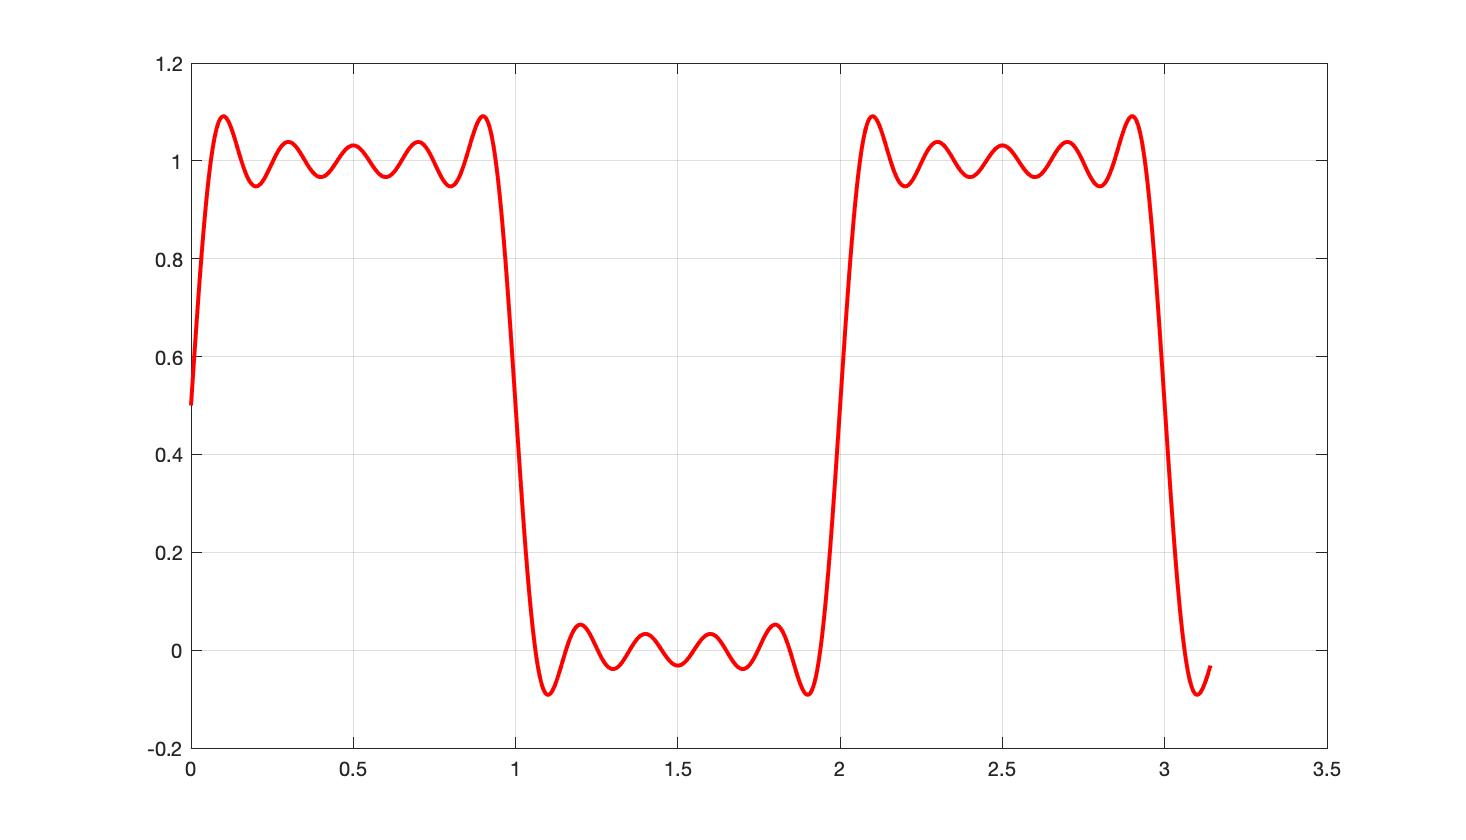
\includegraphics[width=100mm]{Image/Fourier.jpg}
     \end{figure}
     \section{Filter:}
     
     
     
     \cleardoublepage
     \section{Logic Circuits}
     \subsection{Combination of Logic Circuits:}
     \subsubsection{AND Gate:}
     The \textbf{AND} operation on two logic variables, A and B, is represented as AB, read as ``A and B." The \textbf{AND} operation is also called logical multiplication.
     \begin{gather}
         AA=A\\
         A1=A\\
         A0=A\\
         AB=BA\\
         A(BC)=(AB)C=ABC
     \end{gather}
     \begin{figure}[H]
         \centering
         \captionsetup{labelformat=empty}
         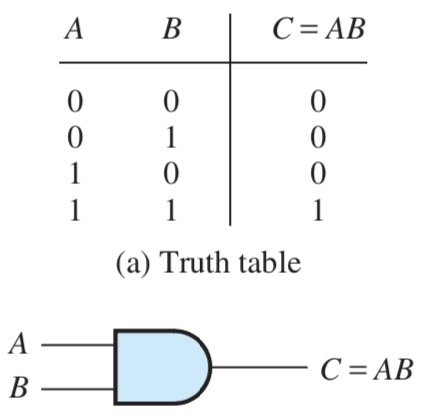
\includegraphics[width=60mm]{Image/35.jpg}
        \caption{Symbol for two-input AND gate}
     \end{figure}
     \subsubsection{Logic Inverteer:}
     The NOT operation on a logic variable is represented by placing a bar over the symbol for the logic variable. 
     \begin{gather}
         A\bar{A}=0\\
       \bar{\bar{A}}=A
     \end{gather}
     \begin{figure}[H]
         \centering
         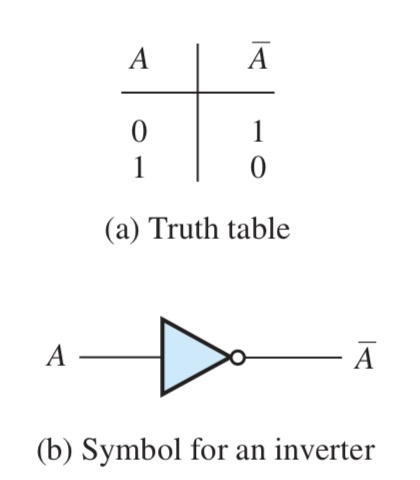
\includegraphics[width=60mm]{Image/36.jpg}
     \end{figure}
     \subsection{OR Gate:}
     The OR operation of logic variables is written as A + B, which is read as ``A or B."
     \begin{gather}
         (A+B)+C=A+(B+C)=A+B+C\\
         A(B+C)=AB+AC\\
         A+0=A\\
         A+1=1\\
         A+\bar{A}=1\\
         A+A=A
     \end{gather}
     \begin{figure}[H]
         \centering
         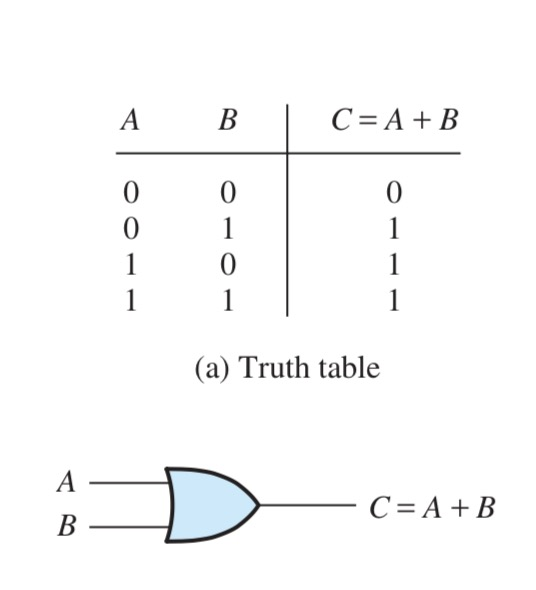
\includegraphics[width=60mm]{Image/37.jpg}
     \end{figure}
     \begin{figure}[H]
         \centering
         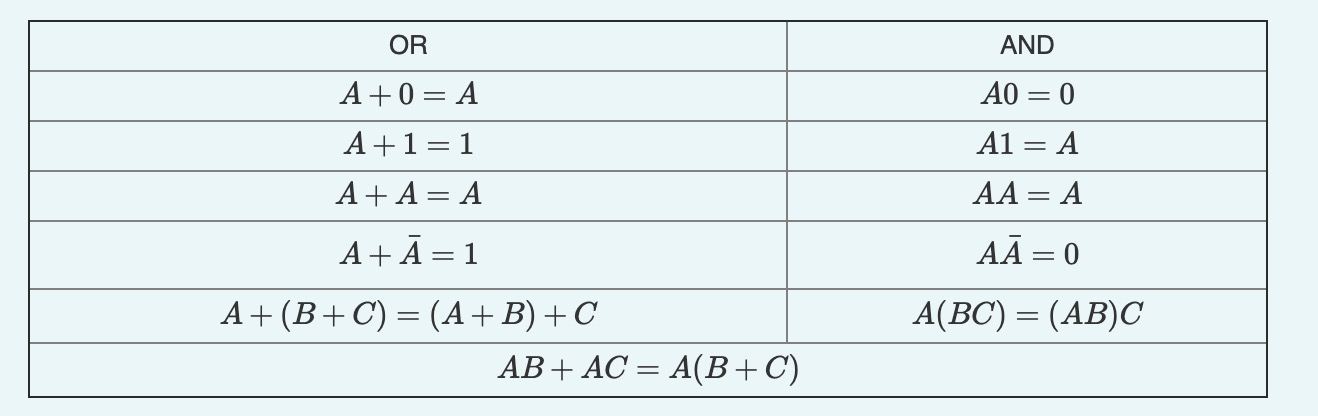
\includegraphics[width=150mm]{Image/39.jpg}
     \end{figure}
     \cleardoublepage
     \textbf{Example:}
     \begin{figure}[H]
         \centering
         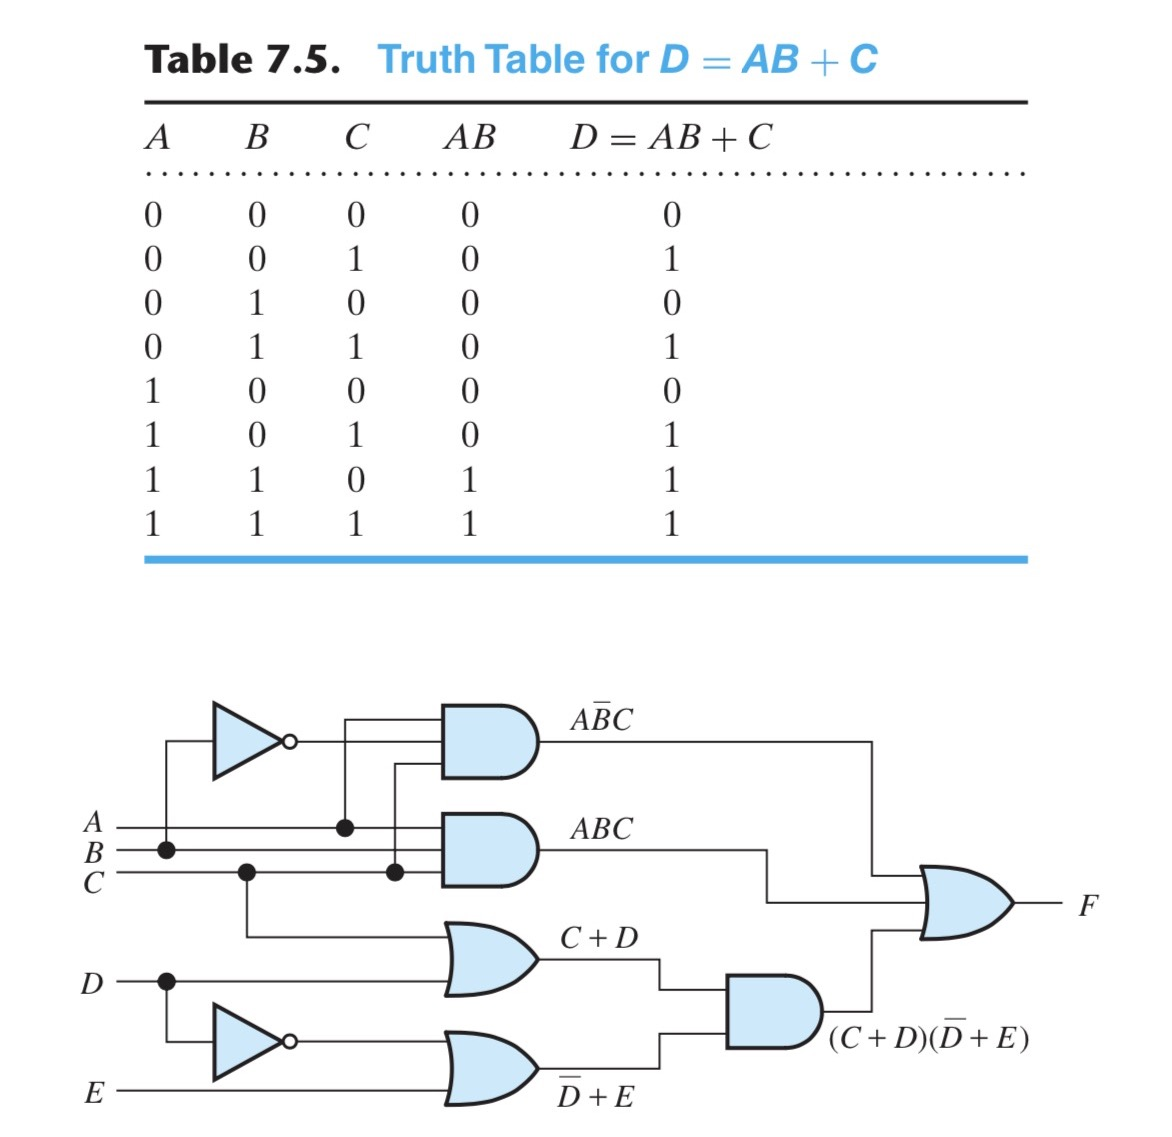
\includegraphics[width=120mm]{Image/38.jpg}
     \end{figure}
     \[F=A\bar{B}C+ABC+(C+D)(\bar{D}+E)\]
     \subsubsection{De Morgan's Laws:}
     Another way to state these laws is as follows: If the variables in a logic expression are replaced by their inverses, the AND operation is replaced by OR, the OR operation is replaced by AND, and the entire expression is inverted, the resulting logic expression yields the same values as before the changes.
     \begin{gather}
         A+B=\overline{\bar{A}+\bar{B}}\\
         AB=\overline{\bar{A}+\bar{B}}
     \end{gather}
     \subsection{SOP(sum of products):}
     \begin{enumerate}
         \item We need concentrate on the rows of the truth table that is 1.
         \item In writing product for each row, we invert the logic variables that are 0 in that row.
         \item Product terms that includes all of the input variables are called minterms.
     \end{enumerate}
     \begin{figure}[H]
         \centering
         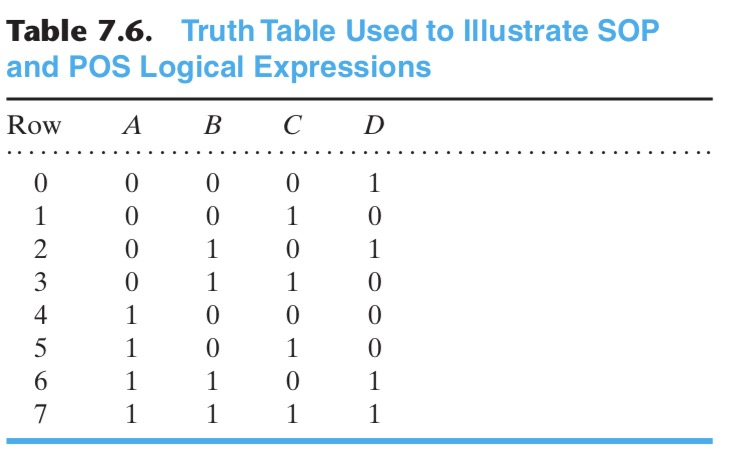
\includegraphics[width=120mm]{Image/40.jpg}
     \end{figure}
     \[D=\bar{A}\bar{B}\bar{C}+\bar{A}B\bar{C}+AB\bar{C}+ABC\]
     \[\sum m(0,2,6,7)\]
     \subsection{POS (product of sum)}
     \begin{enumerate}
         \item identify row with 0 output(Max term)
         \item write logical sum for each one
         \item invert logic variables that are 1 in that row
     \end{enumerate}
     \[D=(A+B+\bar{C})(A+\bar{B}+\bar{C})(\bar{A}+B+C)(\bar{A}+B+\bar{C})\]
     \[D=\Pi M(1,2,3,4,5)\]
     \subsection{Karnaugh Maps:}
     \begin{figure}[H]
         \centering
         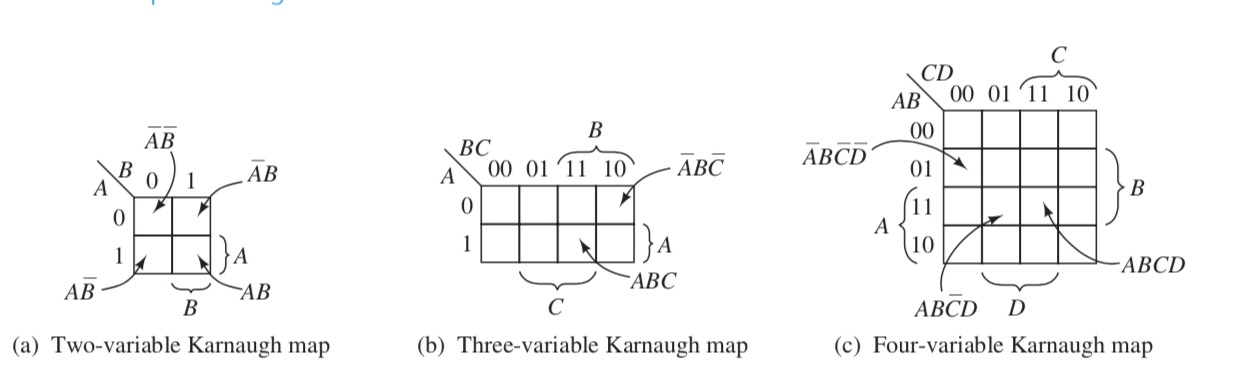
\includegraphics[width=150mm]{Image/41.jpg}
         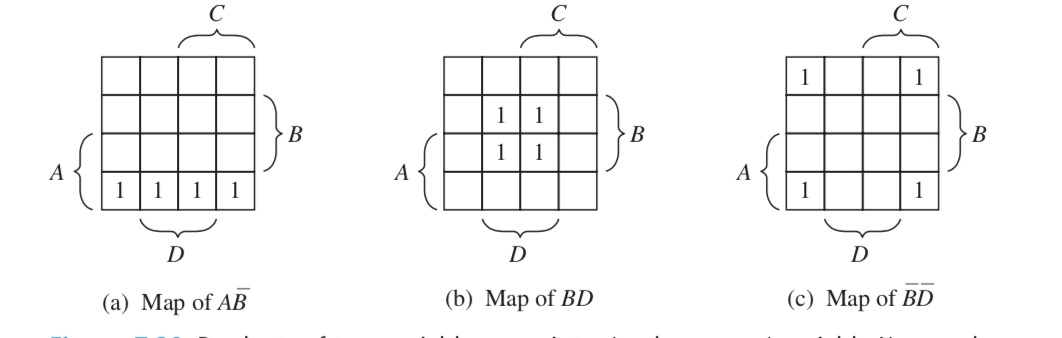
\includegraphics[width=120mm]{Image/42.jpg}
     \end{figure}
     
     \section{Amplifier:}
     \begin{figure}[H]
         \centering
         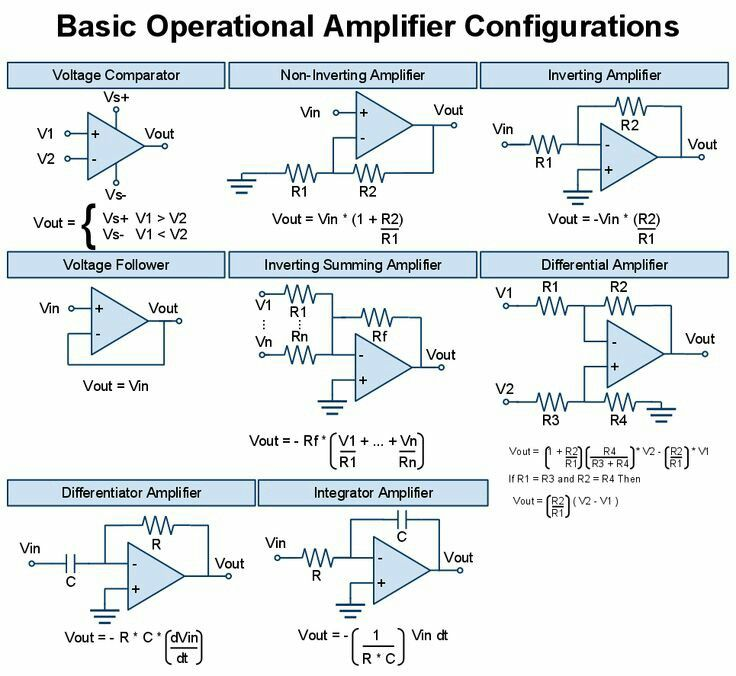
\includegraphics[width=100mm]{Image/Amplifier.jpg}
     \end{figure}
\section{Chapter 9: Review Calpoly}

\begin{align}
    V &=V_m\cos(\omega t+\phi)\\
    V_{rms} &=V_m*\frac{\sqrt{2}}{2}\\
    \sin(\omega t +\theta)&=cos(\omega t+\theta-90^\circ)\\
    \omega &= 2\pi f=\frac{2\pi}{T}\\
    cos(\omega t)+i \sin(\omega t) &=e^{i\omega t}
\end{align}

\cleardoublepage

\section{Chapter 10}
\begin{align*}
    v &=V_m \cos(\omega t +\theta_v-\theta _i)\\
    i &=I_m cos(\omega t)\\
    p &=\begin{cases}
     power &=V_mI_m \cos(\omega t+\theta_v -\theta _i)\cos \omega t\\
    p &=\frac{V_mI_m}{2}cos(\theta _v-\theta _i)+\frac{V_mI_m}{2}cos(\theta _v-\theta _i)cos2\omega t-\frac{V_m I_m}{2}sin(\theta_v-\theta _i)sin2\omega t)\\
    p &=P+Pcos2\omega t-Qsin2\omega t\\
    P_{avg} &=\frac{V_mI_m}{2}cos(\theta_v-\theta _i)\\
   Q_{reactive power} &=\frac{V_mI_m}{2}sin(\theta_v-\theta _i)
    \end{cases}
\end{align*}
\end{document}